% ============================================================================
% UNIVERSAL SPECTRAL LANGUAGE (USL) — Terminology Reference
% Musical Intelligence System — L³ Language Layer
% Version 0.1.0 | 2026-02-14
% ============================================================================

\documentclass[a4paper, 10pt]{article}

% --- Geometry ---
\usepackage[
  top=20mm, bottom=20mm, left=18mm, right=18mm,
  headheight=14pt
]{geometry}

% --- Fonts & Encoding ---
\usepackage[T1]{fontenc}
\usepackage[utf8]{inputenc}
\usepackage{lmodern}
\usepackage{microtype}

% --- Math ---
\usepackage{amsmath}

% --- Tables ---
\usepackage{booktabs}
\usepackage{longtable}
\usepackage{array}
\usepackage{multirow}
\usepackage{makecell}
\usepackage{float}

% --- Colors ---
\usepackage[table,dvipsnames]{xcolor}

% Group colors
\definecolor{grpA}{HTML}{E0F7FA}  % Consonance - cyan
\definecolor{grpB}{HTML}{FFF3E0}  % Energy - orange
\definecolor{grpC}{HTML}{E8F5E9}  % Timbre - green
\definecolor{grpD}{HTML}{FFFDE7}  % Change - yellow
\definecolor{grpE}{HTML}{F3E5F5}  % Interactions - purple
\definecolor{grpF}{HTML}{FFEBEE}  % Pitch-Class - red
\definecolor{grpG}{HTML}{E0F2F1}  % Onset Period - teal
\definecolor{grpH}{HTML}{E3F2FD}  % Spectral Harmony - blue
\definecolor{grpI}{HTML}{FCE4EC}  % Spectral Info - magenta
\definecolor{grpJ}{HTML}{EFEBE9}  % Timbre Ext - brown
\definecolor{grpK}{HTML}{F1F8E9}  % Modulation - olive

% Band colors
\definecolor{bandMicro}{HTML}{E0F7FA}
\definecolor{bandMeso}{HTML}{FFF3E0}
\definecolor{bandMacro}{HTML}{E8F5E9}
\definecolor{bandUltra}{HTML}{F3E5F5}

% Morph category colors
\definecolor{catDist}{HTML}{E0F7FA}
\definecolor{catDyn}{HTML}{FFF3E0}
\definecolor{catRhy}{HTML}{E8F5E9}
\definecolor{catInfo}{HTML}{FCE4EC}
\definecolor{catSym}{HTML}{E3F2FD}

% --- Graphics ---
\usepackage{tikz}
\usetikzlibrary{arrows.meta, positioning, shapes.geometric, calc, fit, backgrounds}

% --- Headers ---
\usepackage{fancyhdr}
\pagestyle{fancy}
\fancyhf{}
\fancyhead[L]{\small\textsc{Universal Spectral Language}}
\fancyhead[R]{\small\textsc{MI System — L³}}
\fancyfoot[C]{\thepage}
\renewcommand{\headrulewidth}{0.4pt}

% --- Hyperlinks ---
\usepackage{hyperref}
\hypersetup{
  colorlinks=true,
  linkcolor=NavyBlue,
  urlcolor=NavyBlue,
  pdftitle={Universal Spectral Language — Terminology Reference},
  pdfauthor={MI Architecture Team}
}

% --- Section formatting ---
\usepackage{titlesec}
\titleformat{\section}{\Large\bfseries\sffamily}{}{0em}{}[\vspace{-0.5em}\rule{\textwidth}{0.8pt}]
\titleformat{\subsection}{\large\bfseries\sffamily}{}{0em}{}

% --- Custom commands ---
\newcommand{\usl}[1]{\texttt{\small #1}}
\newcommand{\legacy}[1]{\texttt{\small\color{gray}#1}}
\newcommand{\addr}[1]{\texttt{\footnotesize\bfseries #1}}
\newcommand{\Rthree}{R\textsuperscript{3}}
\newcommand{\Hthree}{H\textsuperscript{3}}
\newcommand{\Cthree}{C\textsuperscript{3}}
\newcommand{\Lthree}{L\textsuperscript{3}}

% ============================================================================
\begin{document}

% --- Title Page ---
\begin{titlepage}
\centering
\vspace*{3cm}

{\Huge\bfseries\sffamily Universal Spectral Language}\\[0.8cm]
{\LARGE\sffamily Terminology Reference}\\[0.3cm]
{\large\sffamily\color{gray} \Lthree\ — Language Layer}\\[2cm]

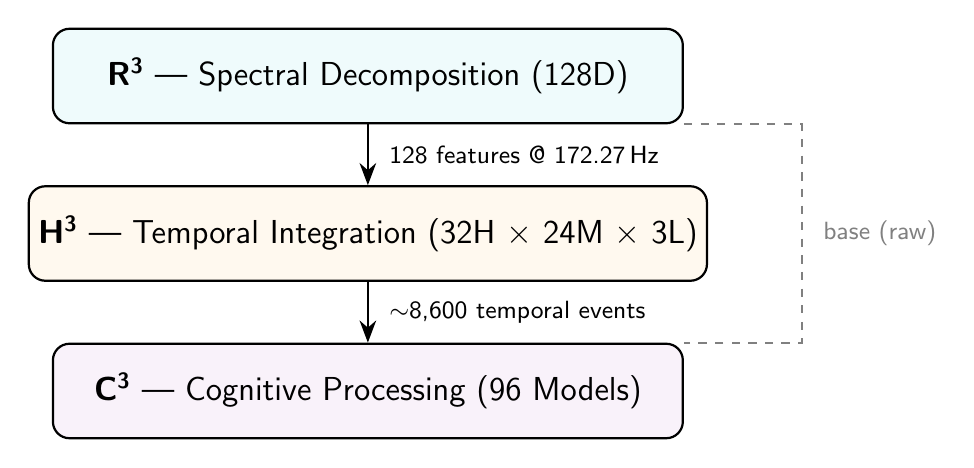
\begin{tikzpicture}[
  layer/.style={draw, rounded corners=6pt, minimum width=8cm, minimum height=1.2cm,
    font=\sffamily\large, thick},
]
  \node[layer, fill=grpA!50] (r3) at (0,0) {\textbf{\Rthree} — Spectral Decomposition (128D)};
  \node[layer, fill=bandMeso!50] (h3) at (0,-2) {\textbf{\Hthree} — Temporal Integration (32H $\times$ 24M $\times$ 3L)};
  \node[layer, fill=grpE!50] (c3) at (0,-4) {\textbf{\Cthree} — Cognitive Processing (96 Models)};

  \draw[-{Stealth[length=8pt]}, thick] (r3.south) -- (h3.north)
    node[midway, right=4pt, font=\small\sffamily] {128 features @ 172.27\,Hz};
  \draw[-{Stealth[length=8pt]}, thick] (h3.south) -- (c3.north)
    node[midway, right=4pt, font=\small\sffamily] {$\sim$8{,}600 temporal events};

  \draw[dashed, thick, gray] (r3.south east) -- ++(1.5,0) |- (c3.north east)
    node[pos=0.25, right=4pt, font=\small\sffamily\color{gray}] {base (raw)};
\end{tikzpicture}

\vspace{2cm}

{\large Version 0.1.0 \quad|\quad 2026-02-14}\\[0.5cm]
{\normalsize Musical Intelligence System}\\[0.3cm]
{\small\color{gray} One system. One language. Spectral.}

\vfill
{\footnotesize\color{gray} This document defines the complete terminological vocabulary\\
used across all layers of the MI system. Every name, every address,\\
every reference follows the conventions defined herein.}
\end{titlepage}

% --- Table of Contents ---
\tableofcontents
\newpage

% --- Core Principle Box ---
\begin{center}
\fcolorbox{NavyBlue}{NavyBlue!5}{%
\begin{minipage}{0.92\textwidth}
\vspace{6pt}
\centering\sffamily
\textbf{\large Core Principle}\\[4pt]
\normalsize
\Rthree\ names describe \textbf{what is measured} (spectral property).\\
\Hthree\ names describe \textbf{how it evolves} (temporal morphology).\\
\Cthree\ models \textbf{interpret} spectral evidence (emergent cognition).\\[4pt]
No music-theory term appears as a computational primitive in \Rthree\ or \Hthree.\\
``Chord'', ``key'', ``cadence'' are \Cthree-emergent concepts.
\vspace{6pt}
\end{minipage}}
\end{center}

\vspace{1em}

% ============================================================================
% SECTION 1: R³
% ============================================================================
% ============================================================================
%  R³ — Spectral Vocabulary (128 Features)
%  Fragment file — % ============================================================================
%  R³ — Spectral Vocabulary (128 Features)
%  Fragment file — % ============================================================================
%  R³ — Spectral Vocabulary (128 Features)
%  Fragment file — \input{sections/r3_tables} from main document
%  Requires: booktabs, longtable, xcolor (with table option), array
% ============================================================================

\section{R\textsuperscript{3} --- Spectral Vocabulary (128 Features)}
\label{sec:r3-tables}

The complete R\textsuperscript{3} spectral representation comprises 128 normalised
features organised into 11 groups (A--K). Each feature is computed per analysis
frame and mapped to $[0,1]$. The \emph{Legacy Name} column shows the original
internal code identifier; the \emph{USL Name} column shows the standardised
Universal Spectral Language identifier used throughout this document.

% Group colours are defined in the main document preamble (grpA..grpK).

{\small
\begin{longtable}{%
  >{\raggedright}p{0.6cm}    % Index
  >{\raggedright}p{1.4cm}    % Group
  >{\ttfamily\raggedright}p{2.8cm}  % Legacy Name
  >{\ttfamily\raggedright}p{3.0cm}  % USL Name
  >{\raggedright}p{5.2cm}           % Spectral Definition
  >{\centering\arraybackslash}p{0.8cm}  % Range
}
\caption{Complete R\textsuperscript{3} feature index (128 dimensions).}
\label{tab:r3-features} \\
\toprule
\textbf{Idx} & \textbf{Group} & \textbf{Legacy Name} & \textbf{USL Name} & \textbf{Spectral Definition} & \textbf{Range} \\
\midrule
\endfirsthead

\multicolumn{6}{l}{\small\emph{Table~\ref{tab:r3-features} continued from previous page}} \\[4pt]
\toprule
\textbf{Idx} & \textbf{Group} & \textbf{Legacy Name} & \textbf{USL Name} & \textbf{Spectral Definition} & \textbf{Range} \\
\midrule
\endhead

\midrule
\multicolumn{6}{r}{\small\emph{Continued on next page}} \\
\endfoot

\bottomrule
\endlastfoot

% ====================================================================
%  GROUP A — Spectral Consonance [0:6]
% ====================================================================
\multicolumn{6}{l}{\cellcolor{grpA}\textbf{Group A: Spectral Consonance {[0:6]}}} \\
\midrule
\rowcolor{grpA}
0 & A & roughness & roughness & Plomp--Levelt critical band interaction & $[0,1]$ \\
\rowcolor{grpA}
1 & A & sethares\_dissonance & sethares\_dissonance & Partial-pair dissonance sum (Sethares 1993) & $[0,1]$ \\
\rowcolor{grpA}
2 & A & helmholtz\_kang & helmholtz\_fusion & Harmonic series alignment index & $[0,1]$ \\
\rowcolor{grpA}
3 & A & stumpf\_fusion & stumpf\_fusion & Perceptual fusion of simultaneous partials & $[0,1]$ \\
\rowcolor{grpA}
4 & A & sensory\_pleasantness & sensory\_pleasantness & Composite spectral smoothness measure & $[0,1]$ \\
\rowcolor{grpA}
5 & A & inharmonicity & inharmonicity & Deviation of partials from harmonic series & $[0,1]$ \\
\rowcolor{grpA}
6 & A & harmonic\_deviation & partial\_deviation & Weighted partial frequency deviation & $[0,1]$ \\

% ====================================================================
%  GROUP B — Spectral Energy [7:11]
% ====================================================================
\midrule
\multicolumn{6}{l}{\cellcolor{grpB}\textbf{Group B: Spectral Energy {[7:11]}}} \\
\midrule
\rowcolor{grpB}
7  & B & amplitude & amplitude & RMS spectral energy & $[0,1]$ \\
\rowcolor{grpB}
8  & B & velocity\_A & amplitude\_velocity & $\mathrm{d}(\text{amplitude})/\mathrm{d}t$ first difference & $[0,1]$ \\
\rowcolor{grpB}
9  & B & acceleration\_A & amplitude\_acceleration & $\mathrm{d}^{2}(\text{amplitude})/\mathrm{d}t^{2}$ second difference & $[0,1]$ \\
\rowcolor{grpB}
10 & B & loudness & loudness & Perceptual loudness (Stevens) & $[0,1]$ \\
\rowcolor{grpB}
11 & B & onset\_strength & onset\_strength & Spectral flux thresholded for onset detection & $[0,1]$ \\

% ====================================================================
%  GROUP C — Spectral Timbre [12:20]
% ====================================================================
\midrule
\multicolumn{6}{l}{\cellcolor{grpC}\textbf{Group C: Spectral Timbre {[12:20]}}} \\
\midrule
\rowcolor{grpC}
12 & C & warmth & spectral\_warmth & Low-frequency spectral energy ratio & $[0,1]$ \\
\rowcolor{grpC}
13 & C & sharpness & spectral\_sharpness & High-frequency weighted centroid (Zwicker) & $[0,1]$ \\
\rowcolor{grpC}
14 & C & tonalness & spectral\_periodicity & Degree of harmonic structure in spectrum & $[0,1]$ \\
\rowcolor{grpC}
15 & C & clarity & spectral\_clarity & Peak-to-average spectral energy ratio & $[0,1]$ \\
\rowcolor{grpC}
16 & C & spectral\_smoothness & spectral\_smoothness & Inverse spectral irregularity & $[0,1]$ \\
\rowcolor{grpC}
17 & C & spectral\_autocorrelation & spectral\_autocorrelation & Spectral self-similarity & $[0,1]$ \\
\rowcolor{grpC}
18 & C & tristimulus1 & tristimulus\_low & Fundamental partial energy ratio & $[0,1]$ \\
\rowcolor{grpC}
19 & C & tristimulus2 & tristimulus\_mid & Partials 2--4 energy ratio & $[0,1]$ \\
\rowcolor{grpC}
20 & C & tristimulus3 & tristimulus\_high & Partials 5+ energy ratio & $[0,1]$ \\

% ====================================================================
%  GROUP D — Spectral Change [21:24]
% ====================================================================
\midrule
\multicolumn{6}{l}{\cellcolor{grpD}\textbf{Group D: Spectral Change {[21:24]}}} \\
\midrule
\rowcolor{grpD}
21 & D & spectral\_flux & spectral\_flux & Frame-to-frame $L^{2}$ spectral distance & $[0,1]$ \\
\rowcolor{grpD}
22 & D & distribution\_entropy & spectral\_entropy & Shannon entropy of spectral distribution & $[0,1]$ \\
\rowcolor{grpD}
23 & D & distribution\_flatness & spectral\_flatness & Geometric/arithmetic mean ratio of spectrum & $[0,1]$ \\
\rowcolor{grpD}
24 & D & distribution\_concentration & spectral\_concentration & Spectral energy concentration measure & $[0,1]$ \\

% ====================================================================
%  GROUP E — Spectral Interactions [25:48]
% ====================================================================
\midrule
\multicolumn{6}{l}{\cellcolor{grpE}\textbf{Group E: Spectral Interactions {[25:48]}}} \\
\midrule
\rowcolor{grpE}
25--32 & E & x\_l0l5\_0\,..\,7 & energy\_consonance\_0\,..\,7 & Energy $\times$ Consonance cross-product (8 dims) & $[0,1]$ \\
\rowcolor{grpE}
33--40 & E & x\_l4l5\_0\,..\,7 & change\_consonance\_0\,..\,7 & Change $\times$ Consonance cross-product (8 dims) & $[0,1]$ \\
\rowcolor{grpE}
41--48 & E & x\_l5l7\_0\,..\,7 & consonance\_timbre\_0\,..\,7 & Consonance $\times$ Timbre cross-product (8 dims) & $[0,1]$ \\

% ====================================================================
%  GROUP F — Pitch-Class Distribution [49:64]
% ====================================================================
\midrule
\multicolumn{6}{l}{\cellcolor{grpF}\textbf{Group F: Pitch-Class Distribution {[49:64]}}} \\
\midrule
\rowcolor{grpF}
49 & F & chroma\_C  & pce\_0  & Spectral energy in pitch class 0 (C) & $[0,1]$ \\
\rowcolor{grpF}
50 & F & chroma\_Db & pce\_1  & Spectral energy in pitch class 1 (C$\sharp$/D$\flat$) & $[0,1]$ \\
\rowcolor{grpF}
51 & F & chroma\_D  & pce\_2  & Spectral energy in pitch class 2 (D) & $[0,1]$ \\
\rowcolor{grpF}
52 & F & chroma\_Eb & pce\_3  & Spectral energy in pitch class 3 (D$\sharp$/E$\flat$) & $[0,1]$ \\
\rowcolor{grpF}
53 & F & chroma\_E  & pce\_4  & Spectral energy in pitch class 4 (E) & $[0,1]$ \\
\rowcolor{grpF}
54 & F & chroma\_F  & pce\_5  & Spectral energy in pitch class 5 (F) & $[0,1]$ \\
\rowcolor{grpF}
55 & F & chroma\_Gb & pce\_6  & Spectral energy in pitch class 6 (F$\sharp$/G$\flat$) & $[0,1]$ \\
\rowcolor{grpF}
56 & F & chroma\_G  & pce\_7  & Spectral energy in pitch class 7 (G) & $[0,1]$ \\
\rowcolor{grpF}
57 & F & chroma\_Ab & pce\_8  & Spectral energy in pitch class 8 (G$\sharp$/A$\flat$) & $[0,1]$ \\
\rowcolor{grpF}
58 & F & chroma\_A  & pce\_9  & Spectral energy in pitch class 9 (A) & $[0,1]$ \\
\rowcolor{grpF}
59 & F & chroma\_Bb & pce\_10 & Spectral energy in pitch class 10 (A$\sharp$/B$\flat$) & $[0,1]$ \\
\rowcolor{grpF}
60 & F & chroma\_B  & pce\_11 & Spectral energy in pitch class 11 (B) & $[0,1]$ \\
\rowcolor{grpF}
61 & F & pitch\_height & spectral\_centroid\_log & $\log_{2}$-weighted spectral centroid & $[0,1]$ \\
\rowcolor{grpF}
62 & F & pitch\_class\_entropy & pce\_entropy & Shannon entropy of 12D PCE distribution & $[0,1]$ \\
\rowcolor{grpF}
63 & F & pitch\_salience & pce\_salience & Peak-to-median ratio in PCE distribution & $[0,1]$ \\
\rowcolor{grpF}
64 & F & inharmonicity\_index & spectral\_inharmonicity & $1 - (\text{PCE peak} / \text{PCE sum})$ & $[0,1]$ \\

% ====================================================================
%  GROUP G — Onset Periodicity [65:74]
% ====================================================================
\midrule
\multicolumn{6}{l}{\cellcolor{grpG}\textbf{Group G: Onset Periodicity {[65:74]}}} \\
\midrule
\rowcolor{grpG}
65 & G & tempo\_estimate & onset\_period & Dominant period in onset autocorrelation & $[0,1]$ \\
\rowcolor{grpG}
66 & G & beat\_strength & onset\_autocorr\_peak & Autocorrelation value at dominant period & $[0,1]$ \\
\rowcolor{grpG}
67 & G & pulse\_clarity & onset\_periodicity\_clarity & Dominant peak / median ratio in onset autocorr & $[0,1]$ \\
\rowcolor{grpG}
68 & G & syncopation\_index & onset\_offbeat\_ratio & Onset energy at off-period positions & $[0,1]$ \\
\rowcolor{grpG}
69 & G & metricality\_index & onset\_subdivision\_depth & Count of significant nested subdivisions & $[0,1]$ \\
\rowcolor{grpG}
70 & G & isochrony\_nPVI & onset\_interval\_regularity & $1 - \text{nPVI}$ of inter-onset intervals & $[0,1]$ \\
\rowcolor{grpG}
71 & G & groove\_index & onset\_bass\_pulse\_product & offbeat $\times$ bass\_energy $\times$ periodicity\_clarity & $[0,1]$ \\
\rowcolor{grpG}
72 & G & event\_density & onset\_density & Onset count per second (normalised) & $[0,1]$ \\
\rowcolor{grpG}
73 & G & tempo\_stability & onset\_period\_stability & $1 - \text{CV}$ of local onset periods & $[0,1]$ \\
\rowcolor{grpG}
74 & G & rhythmic\_regularity & onset\_interval\_entropy\_inv & $1 -$ normalised IOI histogram entropy & $[0,1]$ \\

% ====================================================================
%  GROUP H — Spectral Harmony [75:86]
% ====================================================================
\midrule
\multicolumn{6}{l}{\cellcolor{grpH}\textbf{Group H: Spectral Harmony {[75:86]}}} \\
\midrule
\rowcolor{grpH}
75 & H & key\_clarity & pcp\_correlation\_peak & Max correlation with 24 K--K profiles & $[0,1]$ \\
\rowcolor{grpH}
76 & H & tonnetz\_fifth\_x & pcg\_fifth\_x & Pitch-class geometry: fifths circle $\cos$ & $[0,1]$ \\
\rowcolor{grpH}
77 & H & tonnetz\_fifth\_y & pcg\_fifth\_y & Pitch-class geometry: fifths circle $\sin$ & $[0,1]$ \\
\rowcolor{grpH}
78 & H & tonnetz\_minor\_x & pcg\_minor\_x & Pitch-class geometry: minor-3rd circle $\cos$ & $[0,1]$ \\
\rowcolor{grpH}
79 & H & tonnetz\_minor\_y & pcg\_minor\_y & Pitch-class geometry: minor-3rd circle $\sin$ & $[0,1]$ \\
\rowcolor{grpH}
80 & H & tonnetz\_major\_x & pcg\_major\_x & Pitch-class geometry: major-3rd circle $\cos$ & $[0,1]$ \\
\rowcolor{grpH}
81 & H & tonnetz\_major\_y & pcg\_major\_y & Pitch-class geometry: major-3rd circle $\sin$ & $[0,1]$ \\
\rowcolor{grpH}
82 & H & voice\_leading\_distance & chroma\_l1\_distance & $L^{1}$ norm of successive PCE differences $/\, 2$ & $[0,1]$ \\
\rowcolor{grpH}
83 & H & harmonic\_change & chroma\_frame\_distance & $1 -$ cosine similarity of successive PCE & $[0,1]$ \\
\rowcolor{grpH}
84 & H & tonal\_stability & chroma\_temporal\_consistency & pcp\_corr\_peak $\times$ $(1 -$ smoothed chroma\_dist$)$ & $[0,1]$ \\
\rowcolor{grpH}
85 & H & diatonicity & pcp\_template\_fit & Max fit to diatonic pitch-class template & $[0,1]$ \\
\rowcolor{grpH}
86 & H & syntactic\_irregularity & chroma\_reference\_divergence & KL divergence from best-fit reference profile & $[0,1]$ \\

% ====================================================================
%  GROUP I — Spectral Information [87:93]
% ====================================================================
\midrule
\multicolumn{6}{l}{\cellcolor{grpI}\textbf{Group I: Spectral Information {[87:93]}}} \\
\midrule
\rowcolor{grpI}
87 & I & melodic\_entropy & pce\_transition\_entropy & Entropy of pitch-class transition distribution & $[0,1]$ \\
\rowcolor{grpI}
88 & I & harmonic\_entropy & chroma\_distribution\_divergence & $\mathrm{KL}(\text{PCE}_{t} \,\|\, \text{PCE}_{\text{avg}})$ exponential mapping & $[0,1]$ \\
\rowcolor{grpI}
89 & I & rhythmic\_information\_content & onset\_interval\_surprisal & $-\log(p(\text{IOI}))$ from running IOI histogram & $[0,1]$ \\
\rowcolor{grpI}
90 & I & spectral\_surprise & spectral\_distribution\_divergence & $\mathrm{KL}(\text{mel}_{t} \,\|\, \text{mel}_{\text{avg}})$ exponential mapping & $[0,1]$ \\
\rowcolor{grpI}
91 & I & information\_rate & spectral\_mutual\_information & $\mathrm{MI}(\text{mel}_{t};\, \text{mel}_{t-1}) / \log(128)$ & $[0,1]$ \\
\rowcolor{grpI}
92 & I & predictive\_entropy & spectral\_prediction\_uncertainty & $0.5 \cdot \log(2\pi e \cdot \sigma_{\text{res}}^{2}) / \log(128)$ & $[0,1]$ \\
\rowcolor{grpI}
93 & I & tonal\_ambiguity & pce\_keyed\_entropy & Entropy of $\mathrm{softmax}(\text{K--K corr} \times 5)$ & $[0,1]$ \\

% ====================================================================
%  GROUP J — Spectral Timbre Extended [94:113]
% ====================================================================
\midrule
\multicolumn{6}{l}{\cellcolor{grpJ}\textbf{Group J: Spectral Timbre Extended {[94:113]}}} \\
\midrule
\rowcolor{grpJ}
94--106 & J & mfcc\_1\,..\,13 & mfcc\_1\,..\,mfcc\_13 & DCT-II coefficients of log-mel spectrum (13 dims) & $[0,1]$ \\
\rowcolor{grpJ}
107--113 & J & spectral\_contrast\_1\,..\,7 & spectral\_contrast\_1\,..\,7 & Peak--valley contrast in 7 octave sub-bands & $[0,1]$ \\

% ====================================================================
%  GROUP K — Spectral Modulation [114:127]
% ====================================================================
\midrule
\multicolumn{6}{l}{\cellcolor{grpK}\textbf{Group K: Spectral Modulation {[114:127]}}} \\
\midrule
\rowcolor{grpK}
114 & K & modulation\_0\_5Hz & mod\_energy\_0.5hz & Temporal modulation energy at 0.5\,Hz & $[0,1]$ \\
\rowcolor{grpK}
115 & K & modulation\_1Hz & mod\_energy\_1hz & Temporal modulation energy at 1\,Hz & $[0,1]$ \\
\rowcolor{grpK}
116 & K & modulation\_2Hz & mod\_energy\_2hz & Temporal modulation energy at 2\,Hz & $[0,1]$ \\
\rowcolor{grpK}
117 & K & modulation\_4Hz & mod\_energy\_4hz & Temporal modulation energy at 4\,Hz & $[0,1]$ \\
\rowcolor{grpK}
118 & K & modulation\_8Hz & mod\_energy\_8hz & Temporal modulation energy at 8\,Hz & $[0,1]$ \\
\rowcolor{grpK}
119 & K & modulation\_16Hz & mod\_energy\_16hz & Temporal modulation energy at 16\,Hz & $[0,1]$ \\
\rowcolor{grpK}
120 & K & modulation\_centroid & mod\_centroid & Centroid of modulation spectrum & $[0,1]$ \\
\rowcolor{grpK}
121 & K & modulation\_bandwidth & mod\_bandwidth & Bandwidth of modulation spectrum & $[0,1]$ \\
\rowcolor{grpK}
122 & K & sharpness\_zwicker & sharpness\_zwicker & Zwicker sharpness (Bark-weighted) & $[0,1]$ \\
\rowcolor{grpK}
123 & K & fluctuation\_strength & fluctuation\_strength & Fluctuation strength (4\,Hz peak) & $[0,1]$ \\
\rowcolor{grpK}
124 & K & loudness\_a\_weighted & loudness\_a\_weighted & A-weighted loudness & $[0,1]$ \\
\rowcolor{grpK}
125 & K & alpha\_ratio & alpha\_ratio & Energy ratio below/above 1\,kHz & $[0,1]$ \\
\rowcolor{grpK}
126 & K & hammarberg\_index & hammarberg\_index & Energy peak ratio 0--2\,kHz / 2--5\,kHz & $[0,1]$ \\
\rowcolor{grpK}
127 & K & spectral\_slope\_0\_500 & spectral\_slope\_0\_500 & Linear regression slope of spectrum 0--500\,Hz & $[0,1]$ \\

\end{longtable}
}% end \small
 from main document
%  Requires: booktabs, longtable, xcolor (with table option), array
% ============================================================================

\section{R\textsuperscript{3} --- Spectral Vocabulary (128 Features)}
\label{sec:r3-tables}

The complete R\textsuperscript{3} spectral representation comprises 128 normalised
features organised into 11 groups (A--K). Each feature is computed per analysis
frame and mapped to $[0,1]$. The \emph{Legacy Name} column shows the original
internal code identifier; the \emph{USL Name} column shows the standardised
Universal Spectral Language identifier used throughout this document.

% Group colours are defined in the main document preamble (grpA..grpK).

{\small
\begin{longtable}{%
  >{\raggedright}p{0.6cm}    % Index
  >{\raggedright}p{1.4cm}    % Group
  >{\ttfamily\raggedright}p{2.8cm}  % Legacy Name
  >{\ttfamily\raggedright}p{3.0cm}  % USL Name
  >{\raggedright}p{5.2cm}           % Spectral Definition
  >{\centering\arraybackslash}p{0.8cm}  % Range
}
\caption{Complete R\textsuperscript{3} feature index (128 dimensions).}
\label{tab:r3-features} \\
\toprule
\textbf{Idx} & \textbf{Group} & \textbf{Legacy Name} & \textbf{USL Name} & \textbf{Spectral Definition} & \textbf{Range} \\
\midrule
\endfirsthead

\multicolumn{6}{l}{\small\emph{Table~\ref{tab:r3-features} continued from previous page}} \\[4pt]
\toprule
\textbf{Idx} & \textbf{Group} & \textbf{Legacy Name} & \textbf{USL Name} & \textbf{Spectral Definition} & \textbf{Range} \\
\midrule
\endhead

\midrule
\multicolumn{6}{r}{\small\emph{Continued on next page}} \\
\endfoot

\bottomrule
\endlastfoot

% ====================================================================
%  GROUP A — Spectral Consonance [0:6]
% ====================================================================
\multicolumn{6}{l}{\cellcolor{grpA}\textbf{Group A: Spectral Consonance {[0:6]}}} \\
\midrule
\rowcolor{grpA}
0 & A & roughness & roughness & Plomp--Levelt critical band interaction & $[0,1]$ \\
\rowcolor{grpA}
1 & A & sethares\_dissonance & sethares\_dissonance & Partial-pair dissonance sum (Sethares 1993) & $[0,1]$ \\
\rowcolor{grpA}
2 & A & helmholtz\_kang & helmholtz\_fusion & Harmonic series alignment index & $[0,1]$ \\
\rowcolor{grpA}
3 & A & stumpf\_fusion & stumpf\_fusion & Perceptual fusion of simultaneous partials & $[0,1]$ \\
\rowcolor{grpA}
4 & A & sensory\_pleasantness & sensory\_pleasantness & Composite spectral smoothness measure & $[0,1]$ \\
\rowcolor{grpA}
5 & A & inharmonicity & inharmonicity & Deviation of partials from harmonic series & $[0,1]$ \\
\rowcolor{grpA}
6 & A & harmonic\_deviation & partial\_deviation & Weighted partial frequency deviation & $[0,1]$ \\

% ====================================================================
%  GROUP B — Spectral Energy [7:11]
% ====================================================================
\midrule
\multicolumn{6}{l}{\cellcolor{grpB}\textbf{Group B: Spectral Energy {[7:11]}}} \\
\midrule
\rowcolor{grpB}
7  & B & amplitude & amplitude & RMS spectral energy & $[0,1]$ \\
\rowcolor{grpB}
8  & B & velocity\_A & amplitude\_velocity & $\mathrm{d}(\text{amplitude})/\mathrm{d}t$ first difference & $[0,1]$ \\
\rowcolor{grpB}
9  & B & acceleration\_A & amplitude\_acceleration & $\mathrm{d}^{2}(\text{amplitude})/\mathrm{d}t^{2}$ second difference & $[0,1]$ \\
\rowcolor{grpB}
10 & B & loudness & loudness & Perceptual loudness (Stevens) & $[0,1]$ \\
\rowcolor{grpB}
11 & B & onset\_strength & onset\_strength & Spectral flux thresholded for onset detection & $[0,1]$ \\

% ====================================================================
%  GROUP C — Spectral Timbre [12:20]
% ====================================================================
\midrule
\multicolumn{6}{l}{\cellcolor{grpC}\textbf{Group C: Spectral Timbre {[12:20]}}} \\
\midrule
\rowcolor{grpC}
12 & C & warmth & spectral\_warmth & Low-frequency spectral energy ratio & $[0,1]$ \\
\rowcolor{grpC}
13 & C & sharpness & spectral\_sharpness & High-frequency weighted centroid (Zwicker) & $[0,1]$ \\
\rowcolor{grpC}
14 & C & tonalness & spectral\_periodicity & Degree of harmonic structure in spectrum & $[0,1]$ \\
\rowcolor{grpC}
15 & C & clarity & spectral\_clarity & Peak-to-average spectral energy ratio & $[0,1]$ \\
\rowcolor{grpC}
16 & C & spectral\_smoothness & spectral\_smoothness & Inverse spectral irregularity & $[0,1]$ \\
\rowcolor{grpC}
17 & C & spectral\_autocorrelation & spectral\_autocorrelation & Spectral self-similarity & $[0,1]$ \\
\rowcolor{grpC}
18 & C & tristimulus1 & tristimulus\_low & Fundamental partial energy ratio & $[0,1]$ \\
\rowcolor{grpC}
19 & C & tristimulus2 & tristimulus\_mid & Partials 2--4 energy ratio & $[0,1]$ \\
\rowcolor{grpC}
20 & C & tristimulus3 & tristimulus\_high & Partials 5+ energy ratio & $[0,1]$ \\

% ====================================================================
%  GROUP D — Spectral Change [21:24]
% ====================================================================
\midrule
\multicolumn{6}{l}{\cellcolor{grpD}\textbf{Group D: Spectral Change {[21:24]}}} \\
\midrule
\rowcolor{grpD}
21 & D & spectral\_flux & spectral\_flux & Frame-to-frame $L^{2}$ spectral distance & $[0,1]$ \\
\rowcolor{grpD}
22 & D & distribution\_entropy & spectral\_entropy & Shannon entropy of spectral distribution & $[0,1]$ \\
\rowcolor{grpD}
23 & D & distribution\_flatness & spectral\_flatness & Geometric/arithmetic mean ratio of spectrum & $[0,1]$ \\
\rowcolor{grpD}
24 & D & distribution\_concentration & spectral\_concentration & Spectral energy concentration measure & $[0,1]$ \\

% ====================================================================
%  GROUP E — Spectral Interactions [25:48]
% ====================================================================
\midrule
\multicolumn{6}{l}{\cellcolor{grpE}\textbf{Group E: Spectral Interactions {[25:48]}}} \\
\midrule
\rowcolor{grpE}
25--32 & E & x\_l0l5\_0\,..\,7 & energy\_consonance\_0\,..\,7 & Energy $\times$ Consonance cross-product (8 dims) & $[0,1]$ \\
\rowcolor{grpE}
33--40 & E & x\_l4l5\_0\,..\,7 & change\_consonance\_0\,..\,7 & Change $\times$ Consonance cross-product (8 dims) & $[0,1]$ \\
\rowcolor{grpE}
41--48 & E & x\_l5l7\_0\,..\,7 & consonance\_timbre\_0\,..\,7 & Consonance $\times$ Timbre cross-product (8 dims) & $[0,1]$ \\

% ====================================================================
%  GROUP F — Pitch-Class Distribution [49:64]
% ====================================================================
\midrule
\multicolumn{6}{l}{\cellcolor{grpF}\textbf{Group F: Pitch-Class Distribution {[49:64]}}} \\
\midrule
\rowcolor{grpF}
49 & F & chroma\_C  & pce\_0  & Spectral energy in pitch class 0 (C) & $[0,1]$ \\
\rowcolor{grpF}
50 & F & chroma\_Db & pce\_1  & Spectral energy in pitch class 1 (C$\sharp$/D$\flat$) & $[0,1]$ \\
\rowcolor{grpF}
51 & F & chroma\_D  & pce\_2  & Spectral energy in pitch class 2 (D) & $[0,1]$ \\
\rowcolor{grpF}
52 & F & chroma\_Eb & pce\_3  & Spectral energy in pitch class 3 (D$\sharp$/E$\flat$) & $[0,1]$ \\
\rowcolor{grpF}
53 & F & chroma\_E  & pce\_4  & Spectral energy in pitch class 4 (E) & $[0,1]$ \\
\rowcolor{grpF}
54 & F & chroma\_F  & pce\_5  & Spectral energy in pitch class 5 (F) & $[0,1]$ \\
\rowcolor{grpF}
55 & F & chroma\_Gb & pce\_6  & Spectral energy in pitch class 6 (F$\sharp$/G$\flat$) & $[0,1]$ \\
\rowcolor{grpF}
56 & F & chroma\_G  & pce\_7  & Spectral energy in pitch class 7 (G) & $[0,1]$ \\
\rowcolor{grpF}
57 & F & chroma\_Ab & pce\_8  & Spectral energy in pitch class 8 (G$\sharp$/A$\flat$) & $[0,1]$ \\
\rowcolor{grpF}
58 & F & chroma\_A  & pce\_9  & Spectral energy in pitch class 9 (A) & $[0,1]$ \\
\rowcolor{grpF}
59 & F & chroma\_Bb & pce\_10 & Spectral energy in pitch class 10 (A$\sharp$/B$\flat$) & $[0,1]$ \\
\rowcolor{grpF}
60 & F & chroma\_B  & pce\_11 & Spectral energy in pitch class 11 (B) & $[0,1]$ \\
\rowcolor{grpF}
61 & F & pitch\_height & spectral\_centroid\_log & $\log_{2}$-weighted spectral centroid & $[0,1]$ \\
\rowcolor{grpF}
62 & F & pitch\_class\_entropy & pce\_entropy & Shannon entropy of 12D PCE distribution & $[0,1]$ \\
\rowcolor{grpF}
63 & F & pitch\_salience & pce\_salience & Peak-to-median ratio in PCE distribution & $[0,1]$ \\
\rowcolor{grpF}
64 & F & inharmonicity\_index & spectral\_inharmonicity & $1 - (\text{PCE peak} / \text{PCE sum})$ & $[0,1]$ \\

% ====================================================================
%  GROUP G — Onset Periodicity [65:74]
% ====================================================================
\midrule
\multicolumn{6}{l}{\cellcolor{grpG}\textbf{Group G: Onset Periodicity {[65:74]}}} \\
\midrule
\rowcolor{grpG}
65 & G & tempo\_estimate & onset\_period & Dominant period in onset autocorrelation & $[0,1]$ \\
\rowcolor{grpG}
66 & G & beat\_strength & onset\_autocorr\_peak & Autocorrelation value at dominant period & $[0,1]$ \\
\rowcolor{grpG}
67 & G & pulse\_clarity & onset\_periodicity\_clarity & Dominant peak / median ratio in onset autocorr & $[0,1]$ \\
\rowcolor{grpG}
68 & G & syncopation\_index & onset\_offbeat\_ratio & Onset energy at off-period positions & $[0,1]$ \\
\rowcolor{grpG}
69 & G & metricality\_index & onset\_subdivision\_depth & Count of significant nested subdivisions & $[0,1]$ \\
\rowcolor{grpG}
70 & G & isochrony\_nPVI & onset\_interval\_regularity & $1 - \text{nPVI}$ of inter-onset intervals & $[0,1]$ \\
\rowcolor{grpG}
71 & G & groove\_index & onset\_bass\_pulse\_product & offbeat $\times$ bass\_energy $\times$ periodicity\_clarity & $[0,1]$ \\
\rowcolor{grpG}
72 & G & event\_density & onset\_density & Onset count per second (normalised) & $[0,1]$ \\
\rowcolor{grpG}
73 & G & tempo\_stability & onset\_period\_stability & $1 - \text{CV}$ of local onset periods & $[0,1]$ \\
\rowcolor{grpG}
74 & G & rhythmic\_regularity & onset\_interval\_entropy\_inv & $1 -$ normalised IOI histogram entropy & $[0,1]$ \\

% ====================================================================
%  GROUP H — Spectral Harmony [75:86]
% ====================================================================
\midrule
\multicolumn{6}{l}{\cellcolor{grpH}\textbf{Group H: Spectral Harmony {[75:86]}}} \\
\midrule
\rowcolor{grpH}
75 & H & key\_clarity & pcp\_correlation\_peak & Max correlation with 24 K--K profiles & $[0,1]$ \\
\rowcolor{grpH}
76 & H & tonnetz\_fifth\_x & pcg\_fifth\_x & Pitch-class geometry: fifths circle $\cos$ & $[0,1]$ \\
\rowcolor{grpH}
77 & H & tonnetz\_fifth\_y & pcg\_fifth\_y & Pitch-class geometry: fifths circle $\sin$ & $[0,1]$ \\
\rowcolor{grpH}
78 & H & tonnetz\_minor\_x & pcg\_minor\_x & Pitch-class geometry: minor-3rd circle $\cos$ & $[0,1]$ \\
\rowcolor{grpH}
79 & H & tonnetz\_minor\_y & pcg\_minor\_y & Pitch-class geometry: minor-3rd circle $\sin$ & $[0,1]$ \\
\rowcolor{grpH}
80 & H & tonnetz\_major\_x & pcg\_major\_x & Pitch-class geometry: major-3rd circle $\cos$ & $[0,1]$ \\
\rowcolor{grpH}
81 & H & tonnetz\_major\_y & pcg\_major\_y & Pitch-class geometry: major-3rd circle $\sin$ & $[0,1]$ \\
\rowcolor{grpH}
82 & H & voice\_leading\_distance & chroma\_l1\_distance & $L^{1}$ norm of successive PCE differences $/\, 2$ & $[0,1]$ \\
\rowcolor{grpH}
83 & H & harmonic\_change & chroma\_frame\_distance & $1 -$ cosine similarity of successive PCE & $[0,1]$ \\
\rowcolor{grpH}
84 & H & tonal\_stability & chroma\_temporal\_consistency & pcp\_corr\_peak $\times$ $(1 -$ smoothed chroma\_dist$)$ & $[0,1]$ \\
\rowcolor{grpH}
85 & H & diatonicity & pcp\_template\_fit & Max fit to diatonic pitch-class template & $[0,1]$ \\
\rowcolor{grpH}
86 & H & syntactic\_irregularity & chroma\_reference\_divergence & KL divergence from best-fit reference profile & $[0,1]$ \\

% ====================================================================
%  GROUP I — Spectral Information [87:93]
% ====================================================================
\midrule
\multicolumn{6}{l}{\cellcolor{grpI}\textbf{Group I: Spectral Information {[87:93]}}} \\
\midrule
\rowcolor{grpI}
87 & I & melodic\_entropy & pce\_transition\_entropy & Entropy of pitch-class transition distribution & $[0,1]$ \\
\rowcolor{grpI}
88 & I & harmonic\_entropy & chroma\_distribution\_divergence & $\mathrm{KL}(\text{PCE}_{t} \,\|\, \text{PCE}_{\text{avg}})$ exponential mapping & $[0,1]$ \\
\rowcolor{grpI}
89 & I & rhythmic\_information\_content & onset\_interval\_surprisal & $-\log(p(\text{IOI}))$ from running IOI histogram & $[0,1]$ \\
\rowcolor{grpI}
90 & I & spectral\_surprise & spectral\_distribution\_divergence & $\mathrm{KL}(\text{mel}_{t} \,\|\, \text{mel}_{\text{avg}})$ exponential mapping & $[0,1]$ \\
\rowcolor{grpI}
91 & I & information\_rate & spectral\_mutual\_information & $\mathrm{MI}(\text{mel}_{t};\, \text{mel}_{t-1}) / \log(128)$ & $[0,1]$ \\
\rowcolor{grpI}
92 & I & predictive\_entropy & spectral\_prediction\_uncertainty & $0.5 \cdot \log(2\pi e \cdot \sigma_{\text{res}}^{2}) / \log(128)$ & $[0,1]$ \\
\rowcolor{grpI}
93 & I & tonal\_ambiguity & pce\_keyed\_entropy & Entropy of $\mathrm{softmax}(\text{K--K corr} \times 5)$ & $[0,1]$ \\

% ====================================================================
%  GROUP J — Spectral Timbre Extended [94:113]
% ====================================================================
\midrule
\multicolumn{6}{l}{\cellcolor{grpJ}\textbf{Group J: Spectral Timbre Extended {[94:113]}}} \\
\midrule
\rowcolor{grpJ}
94--106 & J & mfcc\_1\,..\,13 & mfcc\_1\,..\,mfcc\_13 & DCT-II coefficients of log-mel spectrum (13 dims) & $[0,1]$ \\
\rowcolor{grpJ}
107--113 & J & spectral\_contrast\_1\,..\,7 & spectral\_contrast\_1\,..\,7 & Peak--valley contrast in 7 octave sub-bands & $[0,1]$ \\

% ====================================================================
%  GROUP K — Spectral Modulation [114:127]
% ====================================================================
\midrule
\multicolumn{6}{l}{\cellcolor{grpK}\textbf{Group K: Spectral Modulation {[114:127]}}} \\
\midrule
\rowcolor{grpK}
114 & K & modulation\_0\_5Hz & mod\_energy\_0.5hz & Temporal modulation energy at 0.5\,Hz & $[0,1]$ \\
\rowcolor{grpK}
115 & K & modulation\_1Hz & mod\_energy\_1hz & Temporal modulation energy at 1\,Hz & $[0,1]$ \\
\rowcolor{grpK}
116 & K & modulation\_2Hz & mod\_energy\_2hz & Temporal modulation energy at 2\,Hz & $[0,1]$ \\
\rowcolor{grpK}
117 & K & modulation\_4Hz & mod\_energy\_4hz & Temporal modulation energy at 4\,Hz & $[0,1]$ \\
\rowcolor{grpK}
118 & K & modulation\_8Hz & mod\_energy\_8hz & Temporal modulation energy at 8\,Hz & $[0,1]$ \\
\rowcolor{grpK}
119 & K & modulation\_16Hz & mod\_energy\_16hz & Temporal modulation energy at 16\,Hz & $[0,1]$ \\
\rowcolor{grpK}
120 & K & modulation\_centroid & mod\_centroid & Centroid of modulation spectrum & $[0,1]$ \\
\rowcolor{grpK}
121 & K & modulation\_bandwidth & mod\_bandwidth & Bandwidth of modulation spectrum & $[0,1]$ \\
\rowcolor{grpK}
122 & K & sharpness\_zwicker & sharpness\_zwicker & Zwicker sharpness (Bark-weighted) & $[0,1]$ \\
\rowcolor{grpK}
123 & K & fluctuation\_strength & fluctuation\_strength & Fluctuation strength (4\,Hz peak) & $[0,1]$ \\
\rowcolor{grpK}
124 & K & loudness\_a\_weighted & loudness\_a\_weighted & A-weighted loudness & $[0,1]$ \\
\rowcolor{grpK}
125 & K & alpha\_ratio & alpha\_ratio & Energy ratio below/above 1\,kHz & $[0,1]$ \\
\rowcolor{grpK}
126 & K & hammarberg\_index & hammarberg\_index & Energy peak ratio 0--2\,kHz / 2--5\,kHz & $[0,1]$ \\
\rowcolor{grpK}
127 & K & spectral\_slope\_0\_500 & spectral\_slope\_0\_500 & Linear regression slope of spectrum 0--500\,Hz & $[0,1]$ \\

\end{longtable}
}% end \small
 from main document
%  Requires: booktabs, longtable, xcolor (with table option), array
% ============================================================================

\section{R\textsuperscript{3} --- Spectral Vocabulary (128 Features)}
\label{sec:r3-tables}

The complete R\textsuperscript{3} spectral representation comprises 128 normalised
features organised into 11 groups (A--K). Each feature is computed per analysis
frame and mapped to $[0,1]$. The \emph{Legacy Name} column shows the original
internal code identifier; the \emph{USL Name} column shows the standardised
Universal Spectral Language identifier used throughout this document.

% Group colours are defined in the main document preamble (grpA..grpK).

{\small
\begin{longtable}{%
  >{\raggedright}p{0.6cm}    % Index
  >{\raggedright}p{1.4cm}    % Group
  >{\ttfamily\raggedright}p{2.8cm}  % Legacy Name
  >{\ttfamily\raggedright}p{3.0cm}  % USL Name
  >{\raggedright}p{5.2cm}           % Spectral Definition
  >{\centering\arraybackslash}p{0.8cm}  % Range
}
\caption{Complete R\textsuperscript{3} feature index (128 dimensions).}
\label{tab:r3-features} \\
\toprule
\textbf{Idx} & \textbf{Group} & \textbf{Legacy Name} & \textbf{USL Name} & \textbf{Spectral Definition} & \textbf{Range} \\
\midrule
\endfirsthead

\multicolumn{6}{l}{\small\emph{Table~\ref{tab:r3-features} continued from previous page}} \\[4pt]
\toprule
\textbf{Idx} & \textbf{Group} & \textbf{Legacy Name} & \textbf{USL Name} & \textbf{Spectral Definition} & \textbf{Range} \\
\midrule
\endhead

\midrule
\multicolumn{6}{r}{\small\emph{Continued on next page}} \\
\endfoot

\bottomrule
\endlastfoot

% ====================================================================
%  GROUP A — Spectral Consonance [0:6]
% ====================================================================
\multicolumn{6}{l}{\cellcolor{grpA}\textbf{Group A: Spectral Consonance {[0:6]}}} \\
\midrule
\rowcolor{grpA}
0 & A & roughness & roughness & Plomp--Levelt critical band interaction & $[0,1]$ \\
\rowcolor{grpA}
1 & A & sethares\_dissonance & sethares\_dissonance & Partial-pair dissonance sum (Sethares 1993) & $[0,1]$ \\
\rowcolor{grpA}
2 & A & helmholtz\_kang & helmholtz\_fusion & Harmonic series alignment index & $[0,1]$ \\
\rowcolor{grpA}
3 & A & stumpf\_fusion & stumpf\_fusion & Perceptual fusion of simultaneous partials & $[0,1]$ \\
\rowcolor{grpA}
4 & A & sensory\_pleasantness & sensory\_pleasantness & Composite spectral smoothness measure & $[0,1]$ \\
\rowcolor{grpA}
5 & A & inharmonicity & inharmonicity & Deviation of partials from harmonic series & $[0,1]$ \\
\rowcolor{grpA}
6 & A & harmonic\_deviation & partial\_deviation & Weighted partial frequency deviation & $[0,1]$ \\

% ====================================================================
%  GROUP B — Spectral Energy [7:11]
% ====================================================================
\midrule
\multicolumn{6}{l}{\cellcolor{grpB}\textbf{Group B: Spectral Energy {[7:11]}}} \\
\midrule
\rowcolor{grpB}
7  & B & amplitude & amplitude & RMS spectral energy & $[0,1]$ \\
\rowcolor{grpB}
8  & B & velocity\_A & amplitude\_velocity & $\mathrm{d}(\text{amplitude})/\mathrm{d}t$ first difference & $[0,1]$ \\
\rowcolor{grpB}
9  & B & acceleration\_A & amplitude\_acceleration & $\mathrm{d}^{2}(\text{amplitude})/\mathrm{d}t^{2}$ second difference & $[0,1]$ \\
\rowcolor{grpB}
10 & B & loudness & loudness & Perceptual loudness (Stevens) & $[0,1]$ \\
\rowcolor{grpB}
11 & B & onset\_strength & onset\_strength & Spectral flux thresholded for onset detection & $[0,1]$ \\

% ====================================================================
%  GROUP C — Spectral Timbre [12:20]
% ====================================================================
\midrule
\multicolumn{6}{l}{\cellcolor{grpC}\textbf{Group C: Spectral Timbre {[12:20]}}} \\
\midrule
\rowcolor{grpC}
12 & C & warmth & spectral\_warmth & Low-frequency spectral energy ratio & $[0,1]$ \\
\rowcolor{grpC}
13 & C & sharpness & spectral\_sharpness & High-frequency weighted centroid (Zwicker) & $[0,1]$ \\
\rowcolor{grpC}
14 & C & tonalness & spectral\_periodicity & Degree of harmonic structure in spectrum & $[0,1]$ \\
\rowcolor{grpC}
15 & C & clarity & spectral\_clarity & Peak-to-average spectral energy ratio & $[0,1]$ \\
\rowcolor{grpC}
16 & C & spectral\_smoothness & spectral\_smoothness & Inverse spectral irregularity & $[0,1]$ \\
\rowcolor{grpC}
17 & C & spectral\_autocorrelation & spectral\_autocorrelation & Spectral self-similarity & $[0,1]$ \\
\rowcolor{grpC}
18 & C & tristimulus1 & tristimulus\_low & Fundamental partial energy ratio & $[0,1]$ \\
\rowcolor{grpC}
19 & C & tristimulus2 & tristimulus\_mid & Partials 2--4 energy ratio & $[0,1]$ \\
\rowcolor{grpC}
20 & C & tristimulus3 & tristimulus\_high & Partials 5+ energy ratio & $[0,1]$ \\

% ====================================================================
%  GROUP D — Spectral Change [21:24]
% ====================================================================
\midrule
\multicolumn{6}{l}{\cellcolor{grpD}\textbf{Group D: Spectral Change {[21:24]}}} \\
\midrule
\rowcolor{grpD}
21 & D & spectral\_flux & spectral\_flux & Frame-to-frame $L^{2}$ spectral distance & $[0,1]$ \\
\rowcolor{grpD}
22 & D & distribution\_entropy & spectral\_entropy & Shannon entropy of spectral distribution & $[0,1]$ \\
\rowcolor{grpD}
23 & D & distribution\_flatness & spectral\_flatness & Geometric/arithmetic mean ratio of spectrum & $[0,1]$ \\
\rowcolor{grpD}
24 & D & distribution\_concentration & spectral\_concentration & Spectral energy concentration measure & $[0,1]$ \\

% ====================================================================
%  GROUP E — Spectral Interactions [25:48]
% ====================================================================
\midrule
\multicolumn{6}{l}{\cellcolor{grpE}\textbf{Group E: Spectral Interactions {[25:48]}}} \\
\midrule
\rowcolor{grpE}
25--32 & E & x\_l0l5\_0\,..\,7 & energy\_consonance\_0\,..\,7 & Energy $\times$ Consonance cross-product (8 dims) & $[0,1]$ \\
\rowcolor{grpE}
33--40 & E & x\_l4l5\_0\,..\,7 & change\_consonance\_0\,..\,7 & Change $\times$ Consonance cross-product (8 dims) & $[0,1]$ \\
\rowcolor{grpE}
41--48 & E & x\_l5l7\_0\,..\,7 & consonance\_timbre\_0\,..\,7 & Consonance $\times$ Timbre cross-product (8 dims) & $[0,1]$ \\

% ====================================================================
%  GROUP F — Pitch-Class Distribution [49:64]
% ====================================================================
\midrule
\multicolumn{6}{l}{\cellcolor{grpF}\textbf{Group F: Pitch-Class Distribution {[49:64]}}} \\
\midrule
\rowcolor{grpF}
49 & F & chroma\_C  & pce\_0  & Spectral energy in pitch class 0 (C) & $[0,1]$ \\
\rowcolor{grpF}
50 & F & chroma\_Db & pce\_1  & Spectral energy in pitch class 1 (C$\sharp$/D$\flat$) & $[0,1]$ \\
\rowcolor{grpF}
51 & F & chroma\_D  & pce\_2  & Spectral energy in pitch class 2 (D) & $[0,1]$ \\
\rowcolor{grpF}
52 & F & chroma\_Eb & pce\_3  & Spectral energy in pitch class 3 (D$\sharp$/E$\flat$) & $[0,1]$ \\
\rowcolor{grpF}
53 & F & chroma\_E  & pce\_4  & Spectral energy in pitch class 4 (E) & $[0,1]$ \\
\rowcolor{grpF}
54 & F & chroma\_F  & pce\_5  & Spectral energy in pitch class 5 (F) & $[0,1]$ \\
\rowcolor{grpF}
55 & F & chroma\_Gb & pce\_6  & Spectral energy in pitch class 6 (F$\sharp$/G$\flat$) & $[0,1]$ \\
\rowcolor{grpF}
56 & F & chroma\_G  & pce\_7  & Spectral energy in pitch class 7 (G) & $[0,1]$ \\
\rowcolor{grpF}
57 & F & chroma\_Ab & pce\_8  & Spectral energy in pitch class 8 (G$\sharp$/A$\flat$) & $[0,1]$ \\
\rowcolor{grpF}
58 & F & chroma\_A  & pce\_9  & Spectral energy in pitch class 9 (A) & $[0,1]$ \\
\rowcolor{grpF}
59 & F & chroma\_Bb & pce\_10 & Spectral energy in pitch class 10 (A$\sharp$/B$\flat$) & $[0,1]$ \\
\rowcolor{grpF}
60 & F & chroma\_B  & pce\_11 & Spectral energy in pitch class 11 (B) & $[0,1]$ \\
\rowcolor{grpF}
61 & F & pitch\_height & spectral\_centroid\_log & $\log_{2}$-weighted spectral centroid & $[0,1]$ \\
\rowcolor{grpF}
62 & F & pitch\_class\_entropy & pce\_entropy & Shannon entropy of 12D PCE distribution & $[0,1]$ \\
\rowcolor{grpF}
63 & F & pitch\_salience & pce\_salience & Peak-to-median ratio in PCE distribution & $[0,1]$ \\
\rowcolor{grpF}
64 & F & inharmonicity\_index & spectral\_inharmonicity & $1 - (\text{PCE peak} / \text{PCE sum})$ & $[0,1]$ \\

% ====================================================================
%  GROUP G — Onset Periodicity [65:74]
% ====================================================================
\midrule
\multicolumn{6}{l}{\cellcolor{grpG}\textbf{Group G: Onset Periodicity {[65:74]}}} \\
\midrule
\rowcolor{grpG}
65 & G & tempo\_estimate & onset\_period & Dominant period in onset autocorrelation & $[0,1]$ \\
\rowcolor{grpG}
66 & G & beat\_strength & onset\_autocorr\_peak & Autocorrelation value at dominant period & $[0,1]$ \\
\rowcolor{grpG}
67 & G & pulse\_clarity & onset\_periodicity\_clarity & Dominant peak / median ratio in onset autocorr & $[0,1]$ \\
\rowcolor{grpG}
68 & G & syncopation\_index & onset\_offbeat\_ratio & Onset energy at off-period positions & $[0,1]$ \\
\rowcolor{grpG}
69 & G & metricality\_index & onset\_subdivision\_depth & Count of significant nested subdivisions & $[0,1]$ \\
\rowcolor{grpG}
70 & G & isochrony\_nPVI & onset\_interval\_regularity & $1 - \text{nPVI}$ of inter-onset intervals & $[0,1]$ \\
\rowcolor{grpG}
71 & G & groove\_index & onset\_bass\_pulse\_product & offbeat $\times$ bass\_energy $\times$ periodicity\_clarity & $[0,1]$ \\
\rowcolor{grpG}
72 & G & event\_density & onset\_density & Onset count per second (normalised) & $[0,1]$ \\
\rowcolor{grpG}
73 & G & tempo\_stability & onset\_period\_stability & $1 - \text{CV}$ of local onset periods & $[0,1]$ \\
\rowcolor{grpG}
74 & G & rhythmic\_regularity & onset\_interval\_entropy\_inv & $1 -$ normalised IOI histogram entropy & $[0,1]$ \\

% ====================================================================
%  GROUP H — Spectral Harmony [75:86]
% ====================================================================
\midrule
\multicolumn{6}{l}{\cellcolor{grpH}\textbf{Group H: Spectral Harmony {[75:86]}}} \\
\midrule
\rowcolor{grpH}
75 & H & key\_clarity & pcp\_correlation\_peak & Max correlation with 24 K--K profiles & $[0,1]$ \\
\rowcolor{grpH}
76 & H & tonnetz\_fifth\_x & pcg\_fifth\_x & Pitch-class geometry: fifths circle $\cos$ & $[0,1]$ \\
\rowcolor{grpH}
77 & H & tonnetz\_fifth\_y & pcg\_fifth\_y & Pitch-class geometry: fifths circle $\sin$ & $[0,1]$ \\
\rowcolor{grpH}
78 & H & tonnetz\_minor\_x & pcg\_minor\_x & Pitch-class geometry: minor-3rd circle $\cos$ & $[0,1]$ \\
\rowcolor{grpH}
79 & H & tonnetz\_minor\_y & pcg\_minor\_y & Pitch-class geometry: minor-3rd circle $\sin$ & $[0,1]$ \\
\rowcolor{grpH}
80 & H & tonnetz\_major\_x & pcg\_major\_x & Pitch-class geometry: major-3rd circle $\cos$ & $[0,1]$ \\
\rowcolor{grpH}
81 & H & tonnetz\_major\_y & pcg\_major\_y & Pitch-class geometry: major-3rd circle $\sin$ & $[0,1]$ \\
\rowcolor{grpH}
82 & H & voice\_leading\_distance & chroma\_l1\_distance & $L^{1}$ norm of successive PCE differences $/\, 2$ & $[0,1]$ \\
\rowcolor{grpH}
83 & H & harmonic\_change & chroma\_frame\_distance & $1 -$ cosine similarity of successive PCE & $[0,1]$ \\
\rowcolor{grpH}
84 & H & tonal\_stability & chroma\_temporal\_consistency & pcp\_corr\_peak $\times$ $(1 -$ smoothed chroma\_dist$)$ & $[0,1]$ \\
\rowcolor{grpH}
85 & H & diatonicity & pcp\_template\_fit & Max fit to diatonic pitch-class template & $[0,1]$ \\
\rowcolor{grpH}
86 & H & syntactic\_irregularity & chroma\_reference\_divergence & KL divergence from best-fit reference profile & $[0,1]$ \\

% ====================================================================
%  GROUP I — Spectral Information [87:93]
% ====================================================================
\midrule
\multicolumn{6}{l}{\cellcolor{grpI}\textbf{Group I: Spectral Information {[87:93]}}} \\
\midrule
\rowcolor{grpI}
87 & I & melodic\_entropy & pce\_transition\_entropy & Entropy of pitch-class transition distribution & $[0,1]$ \\
\rowcolor{grpI}
88 & I & harmonic\_entropy & chroma\_distribution\_divergence & $\mathrm{KL}(\text{PCE}_{t} \,\|\, \text{PCE}_{\text{avg}})$ exponential mapping & $[0,1]$ \\
\rowcolor{grpI}
89 & I & rhythmic\_information\_content & onset\_interval\_surprisal & $-\log(p(\text{IOI}))$ from running IOI histogram & $[0,1]$ \\
\rowcolor{grpI}
90 & I & spectral\_surprise & spectral\_distribution\_divergence & $\mathrm{KL}(\text{mel}_{t} \,\|\, \text{mel}_{\text{avg}})$ exponential mapping & $[0,1]$ \\
\rowcolor{grpI}
91 & I & information\_rate & spectral\_mutual\_information & $\mathrm{MI}(\text{mel}_{t};\, \text{mel}_{t-1}) / \log(128)$ & $[0,1]$ \\
\rowcolor{grpI}
92 & I & predictive\_entropy & spectral\_prediction\_uncertainty & $0.5 \cdot \log(2\pi e \cdot \sigma_{\text{res}}^{2}) / \log(128)$ & $[0,1]$ \\
\rowcolor{grpI}
93 & I & tonal\_ambiguity & pce\_keyed\_entropy & Entropy of $\mathrm{softmax}(\text{K--K corr} \times 5)$ & $[0,1]$ \\

% ====================================================================
%  GROUP J — Spectral Timbre Extended [94:113]
% ====================================================================
\midrule
\multicolumn{6}{l}{\cellcolor{grpJ}\textbf{Group J: Spectral Timbre Extended {[94:113]}}} \\
\midrule
\rowcolor{grpJ}
94--106 & J & mfcc\_1\,..\,13 & mfcc\_1\,..\,mfcc\_13 & DCT-II coefficients of log-mel spectrum (13 dims) & $[0,1]$ \\
\rowcolor{grpJ}
107--113 & J & spectral\_contrast\_1\,..\,7 & spectral\_contrast\_1\,..\,7 & Peak--valley contrast in 7 octave sub-bands & $[0,1]$ \\

% ====================================================================
%  GROUP K — Spectral Modulation [114:127]
% ====================================================================
\midrule
\multicolumn{6}{l}{\cellcolor{grpK}\textbf{Group K: Spectral Modulation {[114:127]}}} \\
\midrule
\rowcolor{grpK}
114 & K & modulation\_0\_5Hz & mod\_energy\_0.5hz & Temporal modulation energy at 0.5\,Hz & $[0,1]$ \\
\rowcolor{grpK}
115 & K & modulation\_1Hz & mod\_energy\_1hz & Temporal modulation energy at 1\,Hz & $[0,1]$ \\
\rowcolor{grpK}
116 & K & modulation\_2Hz & mod\_energy\_2hz & Temporal modulation energy at 2\,Hz & $[0,1]$ \\
\rowcolor{grpK}
117 & K & modulation\_4Hz & mod\_energy\_4hz & Temporal modulation energy at 4\,Hz & $[0,1]$ \\
\rowcolor{grpK}
118 & K & modulation\_8Hz & mod\_energy\_8hz & Temporal modulation energy at 8\,Hz & $[0,1]$ \\
\rowcolor{grpK}
119 & K & modulation\_16Hz & mod\_energy\_16hz & Temporal modulation energy at 16\,Hz & $[0,1]$ \\
\rowcolor{grpK}
120 & K & modulation\_centroid & mod\_centroid & Centroid of modulation spectrum & $[0,1]$ \\
\rowcolor{grpK}
121 & K & modulation\_bandwidth & mod\_bandwidth & Bandwidth of modulation spectrum & $[0,1]$ \\
\rowcolor{grpK}
122 & K & sharpness\_zwicker & sharpness\_zwicker & Zwicker sharpness (Bark-weighted) & $[0,1]$ \\
\rowcolor{grpK}
123 & K & fluctuation\_strength & fluctuation\_strength & Fluctuation strength (4\,Hz peak) & $[0,1]$ \\
\rowcolor{grpK}
124 & K & loudness\_a\_weighted & loudness\_a\_weighted & A-weighted loudness & $[0,1]$ \\
\rowcolor{grpK}
125 & K & alpha\_ratio & alpha\_ratio & Energy ratio below/above 1\,kHz & $[0,1]$ \\
\rowcolor{grpK}
126 & K & hammarberg\_index & hammarberg\_index & Energy peak ratio 0--2\,kHz / 2--5\,kHz & $[0,1]$ \\
\rowcolor{grpK}
127 & K & spectral\_slope\_0\_500 & spectral\_slope\_0\_500 & Linear regression slope of spectrum 0--500\,Hz & $[0,1]$ \\

\end{longtable}
}% end \small


\newpage

% ============================================================================
% SECTION 2: H³
% ============================================================================
%% H³ Tables — Horizon, Morph, Law
%% \input{} into main document; no preamble.

\section{H\textsuperscript{3} Temporal Demand Space}

% ─────────────────────────────────────────────────────────
\subsection{R\textsuperscript{3} $\to$ H\textsuperscript{3} Dimensional Expansion}
\label{subsec:r3-h3-expansion}

R\textsuperscript{3} produces 128 features per analysis frame at 172.27\,Hz.
Each feature $r_i[t]$ is a \emph{time series}: a sequence of scalar values
across $T$~frames. H\textsuperscript{3} takes these time series and applies
\textbf{temporal morphology}---computing how each spectral property
\emph{behaves over time} at multiple temporal scales.

\paragraph{The four-dimensional demand.}
Every H\textsuperscript{3} output is defined by a 4-tuple:

\begin{center}
\begin{tabular}{@{}rll@{}}
\toprule
\textbf{Component} & \textbf{What it selects} & \textbf{Size} \\
\midrule
\texttt{r3\_idx}  & Which R\textsuperscript{3} feature to observe  & 128 \\
\texttt{horizon}  & How wide a temporal window to use               & 32  \\
\texttt{morph}    & Which statistical descriptor to compute          & 24  \\
\texttt{law}      & Which temporal perspective (causal direction)     & 3   \\
\bottomrule
\end{tabular}
\end{center}

\paragraph{Theoretical vs.\ active space.}
The full Cartesian product yields $128 \times 32 \times 24 \times 3
= \mathbf{294{,}912}$ possible temporal demands.
In practice, each C\textsuperscript{3} model declares only the demands it needs,
yielding $\sim$\textbf{8{,}600 active demands} across all 96 models.

\paragraph{Computation.}
For a given demand $(i, h, m, \ell)$ at frame $t$:

\begin{enumerate}\itemsep2pt
  \item \textbf{Select} the R\textsuperscript{3} feature series: $r_i[t]$.
  \item \textbf{Window} using horizon $h$: extract $n_h$ frames
        according to law $\ell$:
        \begin{itemize}\itemsep1pt
          \item $\ell = \text{L0 (memory)}$: $[t - n_h + 1,\; t]$ \hfill past $\to$ present
          \item $\ell = \text{L1 (prediction)}$: $[t,\; t + n_h - 1]$ \hfill present $\to$ future
          \item $\ell = \text{L2 (integration)}$: $[t - n_h/2,\; t + n_h/2]$ \hfill symmetric
        \end{itemize}
  \item \textbf{Weight} the window with exponential kernel:
        $A(\Delta t) = \exp(-3|\Delta t|/H)$.
  \item \textbf{Apply morph} $m$ to the weighted window
        $\to$ single scalar output.
\end{enumerate}

\paragraph{Output shape.}
Each active demand produces one scalar per frame: the
``temporal morphology'' of that spectral feature at that time scale.
The complete H\textsuperscript{3} output for a given frame is the vector
of all active demand values.

\medskip

% --- TikZ: R³ → H³ expansion diagram ---
\begin{figure}[ht]
\centering
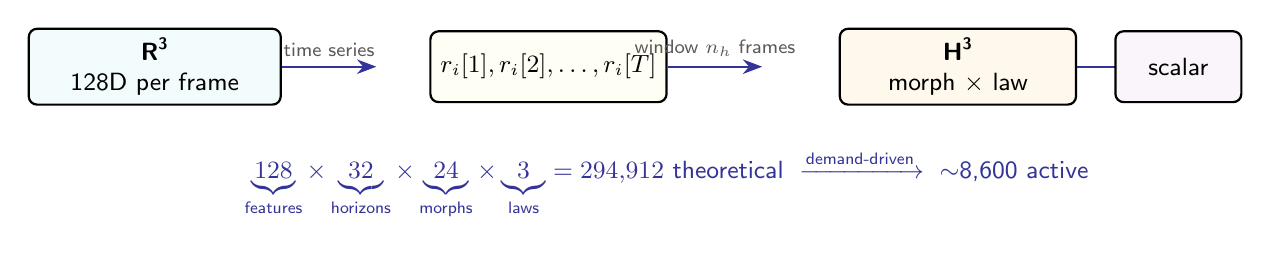
\begin{tikzpicture}[
  box/.style={draw, rounded corners=3pt, minimum height=0.9cm,
    font=\small\sffamily, align=center, thick},
  arr/.style={-{Stealth[length=7pt]}, thick, color=NavyBlue!80},
  brace/.style={decorate, decoration={brace, amplitude=6pt, raise=2pt},
    thick, NavyBlue!70},
  note/.style={font=\scriptsize\sffamily, color=gray!70!black}
]
  % R³ block
  \node[box, fill=grpA!40, minimum width=3.2cm] (r3) at (0, 0)
    {\textbf{R\textsuperscript{3}}\\128D per frame};

  % Arrow
  \draw[arr] (r3.east) -- ++(1.2, 0)
    node[midway, above, note] {time series};

  % Feature series
  \node[box, fill=grpD!40, minimum width=3.0cm] (series) at (5.0, 0)
    {$r_i[1], r_i[2], \ldots, r_i[T]$};

  % Horizon window
  \draw[arr] (series.east) -- ++(1.2, 0)
    node[midway, above, note] {window $n_h$ frames};

  % H³ processing
  \node[box, fill=bandMeso!60, minimum width=3.0cm] (h3) at (10.2, 0)
    {\textbf{H\textsuperscript{3}}\\morph $\times$ law};

  % Output
  \draw[arr] (h3.east) -- ++(1.2, 0);
  \node[box, fill=grpE!40, minimum width=1.6cm] (out) at (13.0, 0)
    {scalar};

  % Bottom: dimensional math
  \node[font=\small\sffamily, text=NavyBlue!80] at (6.5, -1.5)
    {$\underbrace{128}_{\text{features}}
     \times \underbrace{32}_{\text{horizons}}
     \times \underbrace{24}_{\text{morphs}}
     \times \underbrace{3}_{\text{laws}}
     = 294{,}912$ \text{theoretical}
     $\;\xrightarrow{\text{demand-driven}}\;$
     $\sim$8{,}600 \text{active}};
\end{tikzpicture}
\caption{R\textsuperscript{3} $\to$ H\textsuperscript{3} dimensional expansion.
Each R\textsuperscript{3} feature becomes a time series; H\textsuperscript{3}
applies temporal morphology (horizon $\times$ morph $\times$ law) to produce
scalar temporal descriptors. C\textsuperscript{3} models select only the
demands they need from the 294{,}912 theoretical space.}
\label{fig:r3-h3-expansion}
\end{figure}

\paragraph{Concrete example.}
Consider C\textsuperscript{3} model EDNR (Expectancy-Driven Neural Response,
PCU) requesting the demand \addr{83.H12.M9.L0}:

\begin{center}
\small
\begin{tabular}{@{}lll@{}}
\toprule
\textbf{Component} & \textbf{Value} & \textbf{Meaning} \\
\midrule
\texttt{r3\_idx = 83}  & \texttt{chroma\_frame\_distance} & Cosine distance between successive chroma vectors \\
\texttt{horizon = H12} & \texttt{beat} (525\,ms, 90 frames) & Standard beat-level temporal scale \\
\texttt{morph = M9}    & \texttt{velocity\_mean}           & Mean rate of change over the window \\
\texttt{law = L0}      & \texttt{memory} (causal)           & Past $\to$ present: how fast \emph{was} chroma changing \\
\bottomrule
\end{tabular}
\end{center}

\noindent
Result: a single scalar per frame telling EDNR ``the average speed at which
spectral pitch-class distribution changed over the last beat.''

\bigskip

% ─────────────────────────────────────────────────────────
\subsection{H\textsuperscript{3} Output Classification: Named Temporal Properties}
\label{subsec:h3-output-classes}

R\textsuperscript{3} features are raw spectral measurements.
After H\textsuperscript{3} processing, each of the $\sim$8{,}600 active
measurements acquires a \textbf{named temporal identity} at three levels:

\begin{center}
\renewcommand{\arraystretch}{1.2}
\begin{tabular}{@{}rlrl@{}}
\toprule
\textbf{Level} & \textbf{What it names} & \textbf{Count} & \textbf{Example} \\
\midrule
1. Class  & R\textsuperscript{3} Group $\times$ Morph Category & 55
  & \emph{Consonance Motion} \\
2. Type   & Class + specific feature + specific morph & 3{,}072\textsuperscript{*}
  & \emph{roughness velocity} \\
3. Instance & Type + horizon + law & $\sim$8{,}600\textsuperscript{$\dagger$}
  & \texttt{roughness.velocity.beat.memory} \\
\bottomrule
\multicolumn{4}{l}{\scriptsize \textsuperscript{*}128 features $\times$ 24 morphs = 3{,}072 theoretical types.
\textsuperscript{$\dagger$}Demand-driven subset of 294{,}912.}
\end{tabular}
\end{center}

\noindent
The 55 \textbf{classes} (Table~\ref{tab:h3-named-properties}) are the
top-level semantic taxonomy. Each class contains many individual measurements.
For example, the class ``Consonance Level'' spans 7~features $\times$
8~distribution morphs $\times$ up to 32~horizons $\times$ 3~laws.

\medskip

% --- 11×5 Named Temporal Property Matrix ---
{\small
\renewcommand{\arraystretch}{1.15}
\begin{longtable}{@{}
  >{\raggedright}p{1.8cm}
  >{\raggedright}p{2.5cm}
  >{\raggedright}p{2.5cm}
  >{\raggedright}p{2.3cm}
  >{\raggedright}p{2.0cm}
  >{\raggedright\arraybackslash}p{2.3cm}
@{}}
\caption{Level-1 taxonomy: 55 named temporal property classes
(11 R\textsuperscript{3} groups $\times$ 5 morph categories).
Each cell is a \emph{class name} containing many individual measurements.
Horizon and law refine each class into specific Level-3 instances
(e.g.\ ``Consonance Motion'' $\to$ \texttt{roughness.velocity.beat.memory}).}
\label{tab:h3-named-properties} \\
\toprule
\textbf{R\textsuperscript{3} Group}
  & \textbf{Distribution} \newline {\scriptsize M0--M7}
  & \textbf{Dynamics} \newline {\scriptsize M8--M13,15,18,21}
  & \textbf{Periodicity} \newline {\scriptsize M14,17,22}
  & \textbf{Information} \newline {\scriptsize M20}
  & \textbf{Geometry} \newline {\scriptsize M16,19,23} \\
\midrule
\endfirsthead
\toprule
\textbf{R\textsuperscript{3} Group}
  & \textbf{Distribution}
  & \textbf{Dynamics}
  & \textbf{Periodicity}
  & \textbf{Information}
  & \textbf{Geometry} \\
\midrule
\endhead
\midrule
\multicolumn{6}{r}{\footnotesize\itshape continued on next page} \\
\endfoot
\bottomrule
\endlastfoot

\rowcolor{grpA}
\textbf{A} Consonance \newline {\scriptsize [0:6]}
  & Consonance Level
  & Consonance Motion
  & Consonance Periodicity
  & Consonance Predictability
  & Consonance Contour \\[2pt]

\rowcolor{grpB}
\textbf{B} Energy \newline {\scriptsize [7:11]}
  & Energy Level
  & Energy Momentum
  & Energy Pulse
  & Energy Predictability
  & Energy Contour \\[2pt]

\rowcolor{grpC}
\textbf{C} Timbre \newline {\scriptsize [12:20]}
  & Timbre Profile
  & Timbre Drift
  & Timbre Periodicity
  & Timbre Predictability
  & Timbre Contour \\[2pt]

\rowcolor{grpD}
\textbf{D} Change \newline {\scriptsize [21:24]}
  & Change Level
  & Change Acceleration
  & Change Periodicity
  & Change Predictability
  & Change Contour \\[2pt]

\rowcolor{grpE}
\textbf{E} Interactions \newline {\scriptsize [25:48]}
  & Interaction Level
  & Interaction Dynamics
  & Interaction Periodicity
  & Interaction Predictability
  & Interaction Contour \\[2pt]

\rowcolor{grpF}
\textbf{F} Pitch-Class \newline {\scriptsize [49:64]}
  & Pitch-Class Profile
  & Pitch-Class Motion
  & Pitch-Class Periodicity
  & Pitch-Class Predictability
  & Pitch-Class Contour \\[2pt]

\rowcolor{grpG}
\textbf{G} Onset Period \newline {\scriptsize [65:74]}
  & Onset Stability
  & Onset Momentum
  & Onset Regularity
  & Onset Predictability
  & Onset Contour \\[2pt]

\rowcolor{grpH}
\textbf{H} Harmony \newline {\scriptsize [75:86]}
  & Harmonic Stability
  & Harmonic Motion
  & Harmonic Periodicity
  & Harmonic Predictability
  & Harmonic Contour \\[2pt]

\rowcolor{grpI}
\textbf{I} Information \newline {\scriptsize [87:93]}
  & Info Level
  & Info Dynamics
  & Info Periodicity
  & Info Meta-Predictability
  & Info Contour \\[2pt]

\rowcolor{grpJ}
\textbf{J} Timbre Ext. \newline {\scriptsize [94:113]}
  & Texture Profile
  & Texture Drift
  & Texture Periodicity
  & Texture Predictability
  & Texture Contour \\[2pt]

\rowcolor{grpK}
\textbf{K} Modulation \newline {\scriptsize [114:127]}
  & Modulation Level
  & Modulation Dynamics
  & Modulation Periodicity
  & Modulation Predictability
  & Modulation Contour \\

\end{longtable}
}% end \small

\paragraph{Reading the matrix.}
Each cell is a \textbf{named temporal property class}.
Adding a horizon and law makes it fully specific.
Examples:

\begin{center}
\small
\begin{tabular}{@{}llp{7cm}@{}}
\toprule
\textbf{Property Class} & \textbf{Full Address} & \textbf{C\textsuperscript{3} reads as} \\
\midrule
\rowcolor{grpA}
Consonance Level
  & \addr{0.H12.M1.L0}
  & Mean roughness over the last beat (memory) \\[2pt]
\rowcolor{grpA}
Consonance Motion
  & \addr{0.H12.M8.L0}
  & How fast roughness is changing at beat scale \\[2pt]
\rowcolor{grpH}
Harmonic Stability
  & \addr{75.H16.M2.L2}
  & Std.\ dev.\ of key clarity over one measure (integrated) \\[2pt]
\rowcolor{grpH}
Harmonic Periodicity
  & \addr{83.H20.M14.L2}
  & Is chroma distance periodic at phrase scale? \\[2pt]
\rowcolor{grpB}
Energy Momentum
  & \addr{10.H12.M9.L0}
  & Mean velocity of loudness at beat scale (memory) \\[2pt]
\rowcolor{grpG}
Onset Regularity
  & \addr{70.H18.M14.L2}
  & Is onset interval regularity periodic over two measures? \\[2pt]
\rowcolor{grpI}
Info Meta-Predictability
  & \addr{92.H22.M20.L0}
  & Entropy of predictive entropy over a section \\
\bottomrule
\end{tabular}
\end{center}

\paragraph{The naming rule.}
Every H\textsuperscript{3} output name follows:

\begin{center}
\fcolorbox{NavyBlue}{NavyBlue!5}{%
\begin{minipage}{0.88\textwidth}
\centering\sffamily\small
\textbf{H\textsuperscript{3} Temporal Property} =
\textbf{R\textsuperscript{3} Group Name} +
\textbf{Morph Category Name} +
\textbf{Horizon} +
\textbf{Law}\\[4pt]
\normalsize
\texttt{Consonance.Motion.beat.memory} \quad=\quad \addr{0.H12.M8.L0}
\end{minipage}}
\end{center}

\noindent
R\textsuperscript{3} decomposes $\to$ H\textsuperscript{3} names $\to$ C\textsuperscript{3} interprets.

\bigskip

% ─────────────────────────────────────────────────────────
\subsection{H\textsuperscript{3} Horizon Table (32 Temporal Scales)}
\label{tab:h3-horizon}

\begin{longtable}{
  r
  l
  r
  r
  l
  l
}
\toprule
\textbf{Index} & \textbf{USL Label} & \textbf{Duration} & \textbf{Frames} & \textbf{Band} & \textbf{Spectral Scale} \\
\midrule
\endfirsthead

\toprule
\textbf{Index} & \textbf{USL Label} & \textbf{Duration} & \textbf{Frames} & \textbf{Band} & \textbf{Spectral Scale} \\
\midrule
\endhead

\midrule
\multicolumn{6}{r}{\footnotesize\itshape continued on next page} \\
\endfoot

\bottomrule
\endlastfoot

%% Micro band (H0–H7) — cyan!8
\rowcolor{cyan!8}
H0  & \texttt{micro\_0}    & 5.8\,ms    & 1      & Micro & Sub-neural integration     \\
\rowcolor{cyan!8}
H1  & \texttt{micro\_1}    & 11.6\,ms   & 2      & Micro & Neural integration         \\
\rowcolor{cyan!8}
H2  & \texttt{micro\_2}    & 17.4\,ms   & 3      & Micro & Onset detection boundary   \\
\rowcolor{cyan!8}
H3  & \texttt{micro\_3}    & 23.2\,ms   & 4      & Micro & Phoneme boundary           \\
\rowcolor{cyan!8}
H4  & \texttt{micro\_4}    & 34.8\,ms   & 6      & Micro & Pitch period scale         \\
\rowcolor{cyan!8}
H5  & \texttt{micro\_5}    & 46.4\,ms   & 8      & Micro & Pitch integration scale    \\
\rowcolor{cyan!8}
H6  & \texttt{sub\_beat}   & 200\,ms    & 34     & Micro & Sub-beat / note onset      \\
\rowcolor{cyan!8}
H7  & \texttt{short\_note} & 250\,ms    & 43     & Micro & Short note duration        \\

%% Meso band (H8–H15) — orange!8
\rowcolor{orange!8}
H8  & \texttt{eighth}      & 300\,ms    & 52     & Meso  & Eighth-note scale          \\
\rowcolor{orange!8}
H9  & \texttt{fast\_beat}  & 350\,ms    & 60     & Meso  & Fast beat (170\,BPM)       \\
\rowcolor{orange!8}
H10 & \texttt{mod\_beat}   & 400\,ms    & 69     & Meso  & Moderate beat (150\,BPM)   \\
\rowcolor{orange!8}
H11 & \texttt{beat\_low}   & 450\,ms    & 78     & Meso  & Lower beat (130\,BPM)      \\
\rowcolor{orange!8}
H12 & \texttt{beat}        & 525\,ms    & 90     & Meso  & Standard beat (115\,BPM)   \\
\rowcolor{orange!8}
H13 & \texttt{beat\_slow}  & 600\,ms    & 103    & Meso  & Slow beat (100\,BPM)       \\
\rowcolor{orange!8}
H14 & \texttt{dotted}      & 700\,ms    & 121    & Meso  & Dotted quarter scale       \\
\rowcolor{orange!8}
H15 & \texttt{two\_beats}  & 800\,ms    & 138    & Meso  & Two-beat grouping          \\

%% Macro band (H16–H23) — green!8
\rowcolor{green!8}
H16 & \texttt{measure}     & 1{,}000\,ms  & 172    & Macro & Single measure scale       \\
\rowcolor{green!8}
H17 & \texttt{measure\_1h} & 1{,}500\,ms  & 259    & Macro & 1.5 measure scale          \\
\rowcolor{green!8}
H18 & \texttt{two\_meas}   & 2{,}000\,ms  & 345    & Macro & Two-measure scale          \\
\rowcolor{green!8}
H19 & \texttt{three\_meas} & 3{,}000\,ms  & 517    & Macro & Three-measure scale        \\
\rowcolor{green!8}
H20 & \texttt{phrase\_s}   & 5{,}000\,ms  & 861    & Macro & Short phrase (5\,s)        \\
\rowcolor{green!8}
H21 & \texttt{phrase\_l}   & 8{,}000\,ms  & 1{,}378  & Macro & Long phrase (8\,s)         \\
\rowcolor{green!8}
H22 & \texttt{section}     & 15{,}000\,ms & 2{,}584  & Macro & Section (15\,s)            \\
\rowcolor{green!8}
H23 & \texttt{section\_l}  & 25{,}000\,ms & 4{,}307  & Macro & Extended section (25\,s)   \\

%% Ultra band (H24–H31) — purple!8
\rowcolor{purple!8}
H24 & \texttt{movement\_s} & 36\,s      & 6{,}202    & Ultra & Short movement             \\
\rowcolor{purple!8}
H25 & \texttt{one\_min}    & 60\,s      & 10{,}336   & Ultra & One minute                 \\
\rowcolor{purple!8}
H26 & \texttt{two\_min}    & 120\,s     & 20{,}672   & Ultra & Two minutes                \\
\rowcolor{purple!8}
H27 & \texttt{movement\_m} & 200\,s     & 34{,}453   & Ultra & Medium movement            \\
\rowcolor{purple!8}
H28 & \texttt{movement\_l} & 414\,s     & 71{,}319   & Ultra & Standard movement          \\
\rowcolor{purple!8}
H29 & \texttt{movement\_x} & 600\,s     & 103{,}359  & Ultra & Long movement              \\
\rowcolor{purple!8}
H30 & \texttt{form}        & 800\,s     & 137{,}812  & Ultra & Extended form              \\
\rowcolor{purple!8}
H31 & \texttt{full\_work}  & 981\,s     & 168{,}999  & Ultra & Complete work              \\

\end{longtable}


% ─────────────────────────────────────────────────────────
\subsection{H\textsuperscript{3} Morph Table (24 Temporal Descriptors)}
\label{tab:h3-morph}

\begin{longtable}{
  r
  l
  l
  l
  r
  l
}
\toprule
\textbf{Index} & \textbf{USL Name} & \textbf{Formula} & \textbf{Category} & \textbf{Min Frames} & \textbf{Output Range} \\
\midrule
\endfirsthead

\toprule
\textbf{Index} & \textbf{USL Name} & \textbf{Formula} & \textbf{Category} & \textbf{Min Frames} & \textbf{Output Range} \\
\midrule
\endhead

\midrule
\multicolumn{6}{r}{\footnotesize\itshape continued on next page} \\
\endfoot

\bottomrule
\endlastfoot

%% Distribution — cyan!8
\rowcolor{cyan!8}
M0  & \texttt{attn\_mean}    & $\sum(A \cdot x)/\sum(A)$                 & Distribution & 1 & $[0,1]$      \\
\rowcolor{cyan!8}
M1  & \texttt{mean}          & $\sum(x)/N$                               & Distribution & 1 & $[0,1]$      \\
\rowcolor{cyan!8}
M2  & \texttt{std}           & $\sqrt{\mathrm{var}(x)}$                  & Distribution & 2 & $[0,\infty)$ \\
\rowcolor{cyan!8}
M3  & \texttt{median}        & middle value                              & Distribution & 1 & $[0,1]$      \\
\rowcolor{cyan!8}
M4  & \texttt{max}           & $\max(x)$                                 & Distribution & 1 & $[0,1]$      \\
\rowcolor{cyan!8}
M5  & \texttt{range}         & $\max(x) - \min(x)$                       & Distribution & 2 & $[0,1]$      \\
\rowcolor{cyan!8}
M6  & \texttt{skewness}      & $\mu_3 / \sigma^3$                        & Distribution & 3 & $(-\infty,\infty)$ \\
\rowcolor{cyan!8}
M7  & \texttt{kurtosis}      & $\mu_4 / \sigma^4$                        & Distribution & 4 & $[1,\infty)$ \\

%% Dynamics — orange!8
\rowcolor{orange!8}
M8  & \texttt{velocity}      & $dx/dt$                                   & Dynamics     & 2 & $(-\infty,\infty)$ \\
\rowcolor{orange!8}
M9  & \texttt{velocity\_mean} & $\mathrm{mean}(dx/dt)$                   & Dynamics     & 2 & $(-\infty,\infty)$ \\
\rowcolor{orange!8}
M10 & \texttt{velocity\_std}  & $\mathrm{std}(dx/dt)$                    & Dynamics     & 2 & $[0,\infty)$ \\
\rowcolor{orange!8}
M11 & \texttt{acceleration}   & $d^2x/dt^2$                              & Dynamics     & 3 & $(-\infty,\infty)$ \\
\rowcolor{orange!8}
M12 & \texttt{accel\_mean}    & $\mathrm{mean}(d^2x/dt^2)$              & Dynamics     & 3 & $(-\infty,\infty)$ \\
\rowcolor{orange!8}
M13 & \texttt{accel\_std}     & $\mathrm{std}(d^2x/dt^2)$               & Dynamics     & 3 & $[0,\infty)$ \\

%% Rhythm — green!8
\rowcolor{green!8}
M14 & \texttt{periodicity}    & $\max(\mathrm{autocorr}[\mathrm{lag}>0])$ & Rhythm       & 4 & $[0,1]$      \\

%% Dynamics (continued) — orange!8
\rowcolor{orange!8}
M15 & \texttt{smoothness}     & $1/(1+|\mathrm{jerk}|/\sigma)$           & Dynamics     & 3 & $(0,1]$      \\

%% Symmetry — blue!8
\rowcolor{blue!8}
M16 & \texttt{curvature}      & $\mathrm{mean}(|d^2x/dt^2|)$            & Symmetry     & 3 & $[0,\infty)$ \\

%% Rhythm — green!8
\rowcolor{green!8}
M17 & \texttt{shape\_period}  & velocity zero-crossing $\Delta$           & Rhythm       & 4 & $[0,\infty)$ \\

%% Dynamics (continued) — orange!8
\rowcolor{orange!8}
M18 & \texttt{trend}          & OLS regression slope                      & Dynamics     & 2 & $(-\infty,\infty)$ \\

%% Symmetry — blue!8
\rowcolor{blue!8}
M19 & \texttt{stability}      & $1/(1+\mathrm{var}/\sigma^2)$            & Symmetry     & 2 & $(0,1]$      \\

%% Information — magenta!8
\rowcolor{magenta!8}
M20 & \texttt{entropy}        & $-\Sigma\, p \cdot \log(p)\;/\;\log(16)$ & Information  & 4 & $[0,1]$      \\

%% Dynamics (continued) — orange!8
\rowcolor{orange!8}
M21 & \texttt{zero\_cross}    & sign-change count                         & Dynamics     & 2 & $[0, N{-}1]$ \\

%% Rhythm — green!8
\rowcolor{green!8}
M22 & \texttt{peaks}          & local maxima count                        & Rhythm       & 3 & $[0, N{-}2]$ \\

%% Symmetry — blue!8
\rowcolor{blue!8}
M23 & \texttt{symmetry}       & $\mathrm{corr}(x, \mathrm{reverse}(x))$  & Symmetry     & 2 & $[-1,1]$     \\

\end{longtable}


% ─────────────────────────────────────────────────────────
\subsection{H\textsuperscript{3} Law Table (3 Temporal Perspectives)}
\label{tab:h3-law}

\begin{table}[H]
\centering
\begin{tabular}{r l l l l}
\toprule
\textbf{Index} & \textbf{USL Name} & \textbf{Direction} & \textbf{Kernel} & \textbf{Window} \\
\midrule
L0 & \texttt{memory}      & Past $\to$ Present   & $A(dt) = \exp(-3|dt|/H)$, causal       & $[t{-}n{+}1,\; t]$     \\
L1 & \texttt{prediction}  & Present $\to$ Future  & $A(dt) = \exp(-3|dt|/H)$, anti-causal  & $[t,\; t{+}n{-}1]$     \\
L2 & \texttt{integration} & Past $\leftrightarrow$ Future & $A(dt) = \exp(-3|dt|/H)$, symmetric    & $[t{-}n/2,\; t{+}n/2]$ \\
\bottomrule
\end{tabular}
\end{table}


\newpage

% ============================================================================
% SECTION 3: Address System + C³ Interface
% ============================================================================
% c3_address.tex — C³ Address System and Unit Interface
% Fragment file: % c3_address.tex — C³ Address System and Unit Interface
% Fragment file: % c3_address.tex — C³ Address System and Unit Interface
% Fragment file: \input{sections/c3_address} from main document
% Requires: tikz, booktabs, array, xcolor

%% ============================================================
%%  SECTION 1 — Universal Spectral Address System
%% ============================================================
\section{Universal Spectral Address System}
\label{sec:spectral-address}

Every datum flowing through the MI pipeline carries a \emph{spectral address}:
a four-component tuple that uniquely identifies its origin in the
R\textsuperscript{3}--H\textsuperscript{3} feature--temporal lattice.

\medskip

\begin{center}
\texttt{\{r3\_idx\}.\{horizon\}.\{morph\}.\{law\}}
\end{center}

\medskip

\noindent
\textbf{Numeric example:}\quad \texttt{83.H12.M9.L0}\\[2pt]
\textbf{Spectral label:}\quad
\texttt{chroma\_frame\_distance.beat.velocity\_mean.memory}

% ---- TikZ address decomposition diagram ----
\begin{figure}[ht]
\centering
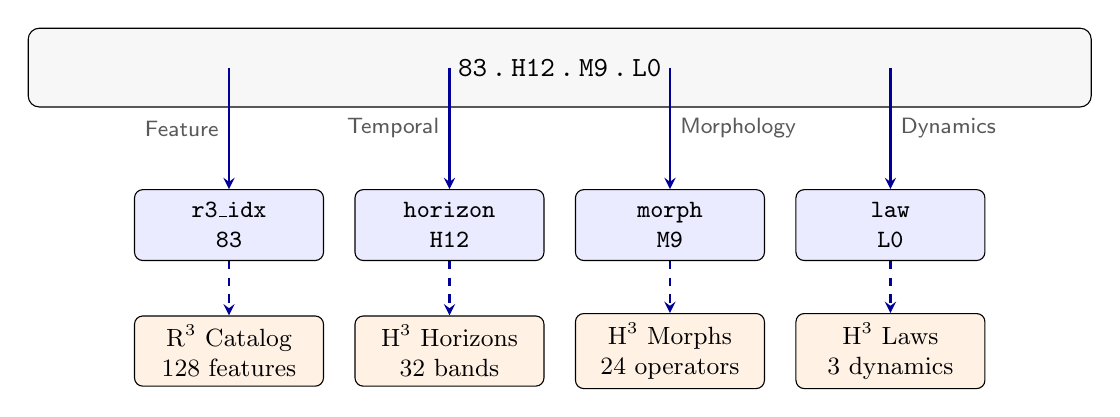
\begin{tikzpicture}[
    comp/.style={
        draw, rounded corners=3pt, fill=blue!8,
        minimum width=2.4cm, minimum height=0.9cm,
        font=\small\ttfamily, align=center
    },
    catalog/.style={
        draw, rounded corners=3pt, fill=orange!10,
        minimum width=2.4cm, minimum height=0.7cm,
        font=\small, align=center
    },
    arr/.style={->, >=stealth, thick, color=blue!60!black},
    lbl/.style={font=\footnotesize\sffamily, color=gray!70!black}
]
    % Full address bar
    \node[draw, rounded corners=4pt, fill=gray!6,
          minimum width=13.5cm, minimum height=1.0cm,
          font=\ttfamily]
        (addr) at (0,0) {83\,.\,H12\,.\,M9\,.\,L0};

    % Invisible anchors for the four segments
    \coordinate (a1) at (-4.2, 0);
    \coordinate (a2) at (-1.4, 0);
    \coordinate (a3) at ( 1.4, 0);
    \coordinate (a4) at ( 4.2, 0);

    % Component boxes below
    \node[comp] (c1) at (-4.2,-2.0) {r3\_idx\\83};
    \node[comp] (c2) at (-1.4,-2.0) {horizon\\H12};
    \node[comp] (c3) at ( 1.4,-2.0) {morph\\M9};
    \node[comp] (c4) at ( 4.2,-2.0) {law\\L0};

    % Arrows from address bar to components
    \draw[arr] (a1) -- (c1) node[midway, left, lbl] {Feature};
    \draw[arr] (a2) -- (c2) node[midway, left, lbl] {Temporal};
    \draw[arr] (a3) -- (c3) node[midway, right, lbl] {Morphology};
    \draw[arr] (a4) -- (c4) node[midway, right, lbl] {Dynamics};

    % Catalog / source layer below components
    \node[catalog] (s1) at (-4.2,-3.6) {R\textsuperscript{3} Catalog\\128 features};
    \node[catalog] (s2) at (-1.4,-3.6) {H\textsuperscript{3} Horizons\\32 bands};
    \node[catalog] (s3) at ( 1.4,-3.6) {H\textsuperscript{3} Morphs\\24 operators};
    \node[catalog] (s4) at ( 4.2,-3.6) {H\textsuperscript{3} Laws\\3 dynamics};

    \draw[arr, dashed] (c1) -- (s1);
    \draw[arr, dashed] (c2) -- (s2);
    \draw[arr, dashed] (c3) -- (s3);
    \draw[arr, dashed] (c4) -- (s4);
\end{tikzpicture}
\caption{Four-tuple spectral address decomposition.
         Each component maps to a specific catalog layer in the
         R\textsuperscript{3}/H\textsuperscript{3} system.}
\label{fig:address-decomposition}
\end{figure}


% ---- Address Construction Rules table ----
\subsection{Address Construction Rules}
\label{subsec:address-rules}

\begin{table}[ht]
\centering
\caption{Address component construction rules.}
\label{tab:address-construction}
\begin{tabular}{@{}llll@{}}
\toprule
\textbf{Component} & \textbf{Source} & \textbf{Range} & \textbf{Example} \\
\midrule
\texttt{r3\_idx} & R\textsuperscript{3} Feature Index & 0--127  & 83  \\
\texttt{horizon} & H\textsuperscript{3} Horizon Index  & H0--H31 & H12 \\
\texttt{morph}   & H\textsuperscript{3} Morph Index    & M0--M23 & M9  \\
\texttt{law}     & H\textsuperscript{3} Law Index      & L0--L2  & L0  \\
\bottomrule
\end{tabular}
\end{table}


% ---- Spectral Label Construction table ----
\subsection{Spectral Label Construction}
\label{subsec:spectral-label}

\begin{table}[ht]
\centering
\caption{Spectral label construction from address components.}
\label{tab:spectral-label}
\begin{tabular}{@{}lll@{}}
\toprule
\textbf{Component} & \textbf{Format} & \textbf{Example} \\
\midrule
Feature    & R\textsuperscript{3} USL name   & \texttt{chroma\_frame\_distance} \\
Horizon    & H\textsuperscript{3} USL label  & \texttt{beat}                   \\
Morph      & H\textsuperscript{3} morph name & \texttt{velocity\_mean}         \\
Law        & H\textsuperscript{3} law name   & \texttt{memory}                 \\
\midrule
Full label & \texttt{feature.horizon.morph.law}
           & \texttt{chroma\_frame\_distance.beat.velocity\_mean.memory} \\
\bottomrule
\end{tabular}
\end{table}


%% ============================================================
%%  SECTION 2 — C³ Unit Interface Table
%% ============================================================
\section{C\textsuperscript{3} Unit Interface Table}
\label{sec:c3-units}

Table~\ref{tab:c3-units} lists all nine C\textsuperscript{3} processing units
and their primary interfaces with the R\textsuperscript{3} feature groups and
H\textsuperscript{3} temporal bands.
R\textsuperscript{3} groups are identified by letter
(A~=~Consonance, B~=~Energy, C~=~Timbre, D~=~Change, E~=~Interactions,
 F~=~Pitch-Class, G~=~Onset Period, H~=~Harmony, I~=~Information,
 J~=~Timbre Ext., K~=~Modulation).
H\textsuperscript{3} bands span Micro ($<$50\,ms), Meso (50\,ms--2\,s),
and Macro ($>$2\,s) perceptual time scales.

\begin{table}[ht]
\centering
\caption{C\textsuperscript{3} unit interface summary.}
\label{tab:c3-units}
\renewcommand{\arraystretch}{1.15}
\begin{tabular}{@{}llclll@{}}
\toprule
\textbf{Unit} & \textbf{Full Name}
  & \textbf{Models}
  & \textbf{Primary R\textsuperscript{3} Groups}
  & \textbf{Primary H\textsuperscript{3} Bands}
  & \textbf{Primary Laws} \\
\midrule
SPU & Sensory Processing    &  9 & A, B, C, D & Micro--Meso  & L0, L2        \\
STU & Structural Timing     & 20 & G, H, I    & Meso--Macro  & L0, L1, L2    \\
IMU & Integrative Memory    & 10 & F, H, I    & Meso--Macro  & L0, L2        \\
ASU & Auditory Scene        &  9 & A, B, C    & Micro--Meso  & L2            \\
NDU & Neuromodulation       &  8 & B, H, I    & Meso--Macro  & L0, L1, L2    \\
MPU & Motor Planning        & 11 & G, H       & Meso         & L0, L1        \\
PCU & Predictive Coding     & 10 & F, H, I    & Micro--Macro & L0, L1, L2    \\
ARU & Arousal Regulation    &  9 & B, H, I    & Meso--Macro  & L0, L1, L2    \\
RPU & Reward Processing     & 10 & H, I, K    & Meso--Macro  & L0, L1, L2    \\
\bottomrule
\end{tabular}
\end{table}


%% ============================================================
%%  SECTION 3 — Provenance Chain Diagram
%% ============================================================
\section{Provenance Chain}
\label{sec:provenance-chain}

Figure~\ref{fig:provenance} traces the complete data-flow from raw audio
to the C\textsuperscript{3} input package.  Every tensor element retains a
spectral address linking it back to its R\textsuperscript{3} source through
an unbroken provenance chain.

\begin{figure}[ht]
\centering
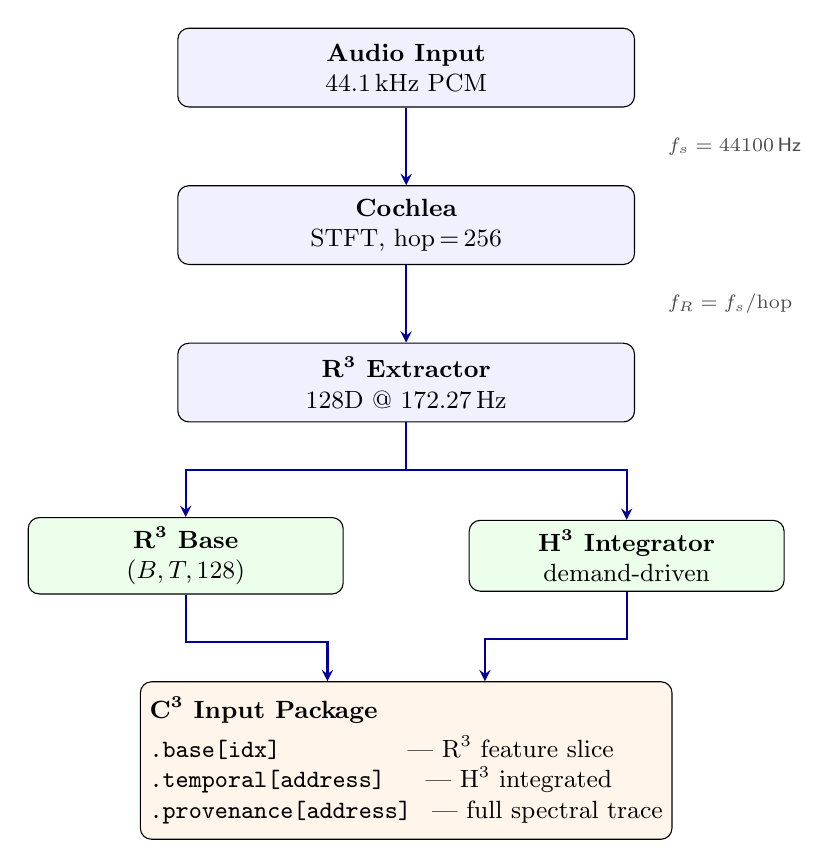
\begin{tikzpicture}[
    block/.style={
        draw, rounded corners=4pt, fill=blue!6,
        minimum width=5.8cm, minimum height=1.0cm,
        font=\small, align=center
    },
    split/.style={
        draw, rounded corners=4pt, fill=green!8,
        minimum width=4.0cm, minimum height=0.9cm,
        font=\small, align=center
    },
    pkg/.style={
        draw, rounded corners=4pt, fill=orange!8,
        minimum width=6.4cm, minimum height=2.0cm,
        font=\small, align=left
    },
    arr/.style={->, >=stealth, thick, color=blue!60!black},
    note/.style={font=\scriptsize\sffamily, color=gray!60!black}
]
    % Top: Audio input
    \node[block] (audio) at (0, 0)
        {\textbf{Audio Input}\\44.1\,kHz PCM};

    % Cochlea
    \node[block] (cochlea) at (0, -2.0)
        {\textbf{Cochlea}\\STFT, hop\,=\,256};
    \draw[arr] (audio) -- (cochlea);
    \node[note, right] at (3.2, -1.0) {$f_s = 44100$\,Hz};

    % R³ Extractor
    \node[block] (r3ext) at (0, -4.0)
        {\textbf{R\textsuperscript{3} Extractor}\\128D @ 172.27\,Hz};
    \draw[arr] (cochlea) -- (r3ext);
    \node[note, right] at (3.2, -3.0) {$f_R = f_s / \mathrm{hop}$};

    % Split into two branches
    \node[split] (r3base) at (-2.8, -6.2)
        {\textbf{R\textsuperscript{3} Base}\\$(B, T, 128)$};
    \node[split] (h3int)  at ( 2.8, -6.2)
        {\textbf{H\textsuperscript{3} Integrator}\\demand-driven};

    \draw[arr] (r3ext.south) -- ++(0,-0.6) -| (r3base.north);
    \draw[arr] (r3ext.south) -- ++(0,-0.6) -| (h3int.north);

    % C³ Input Package
    \node[pkg] (c3pkg) at (0, -8.8)
        {\textbf{C\textsuperscript{3} Input Package}\\[3pt]
         \texttt{.base[idx]}
         \hspace{1.4cm} \textrm{--- R\textsuperscript{3} feature slice}\\
         \texttt{.temporal[address]}
         \hspace{0.3cm} \textrm{--- H\textsuperscript{3} integrated}\\
         \texttt{.provenance[address]}
         \hspace{0.05cm} \textrm{--- full spectral trace}};

    \draw[arr] (r3base.south)  -- ++(0,-0.6) -| ([xshift=-1cm]c3pkg.north);
    \draw[arr] (h3int.south)   -- ++(0,-0.6) -| ([xshift= 1cm]c3pkg.north);
\end{tikzpicture}
\caption{Provenance chain from audio input to C\textsuperscript{3} input package.
         Every tensor element traces back to its R\textsuperscript{3} source
         through spectral addresses.}
\label{fig:provenance}
\end{figure}


%% ============================================================
%%  SECTION 4 — Naming Convention Rules
%% ============================================================
\section{Naming Convention Rules}
\label{sec:naming-rules}

The following rules govern all naming within the Universal Spectral Language.
Violations break the provenance chain and are treated as specification errors.

\begin{enumerate}
    \item \textbf{Measurement, not interpretation.}\enspace
          R\textsuperscript{3} feature names describe what is \emph{measured}
          (e.g.\ \texttt{spectral\_centroid}), never what is
          \emph{perceived} or \emph{interpreted}.

    \item \textbf{No music-theory terms in R\textsuperscript{3}/H\textsuperscript{3}.}\enspace
          Names must not contain \texttt{chord}, \texttt{key},
          \texttt{cadence}, \texttt{tonal}, or \texttt{harmonic}
          in their music-theoretic senses.
          \texttt{harmonic} is permitted only in its signal-processing
          meaning (integer-multiple partials).

    \item \textbf{Perceptual time scales, not musical structure.}\enspace
          H\textsuperscript{3} horizon labels denote perceptual durations.
          For example, \texttt{beat} designates the ${\sim}525$\,ms
          periodicity band, not a musical beat or metrical position.

    \item \textbf{Dot-separated addresses.}\enspace
          Full spectral addresses use dot separation:
          \texttt{feature.horizon.morph.law}.
          No spaces, no slashes, no camelCase.

    \item \textbf{C\textsuperscript{3} music-theory mapping.}\enspace
          C\textsuperscript{3} model documentation \emph{may} reference
          music-theory terms for explanatory purposes, but every such
          reference \emph{must} map to one or more spectral addresses.

    \item \textbf{Unbroken spectral chain.}\enspace
          Every C\textsuperscript{3} input must trace back to an
          R\textsuperscript{3} source through the address system.
          No datum enters C\textsuperscript{3} without a provenance record.
\end{enumerate}
 from main document
% Requires: tikz, booktabs, array, xcolor

%% ============================================================
%%  SECTION 1 — Universal Spectral Address System
%% ============================================================
\section{Universal Spectral Address System}
\label{sec:spectral-address}

Every datum flowing through the MI pipeline carries a \emph{spectral address}:
a four-component tuple that uniquely identifies its origin in the
R\textsuperscript{3}--H\textsuperscript{3} feature--temporal lattice.

\medskip

\begin{center}
\texttt{\{r3\_idx\}.\{horizon\}.\{morph\}.\{law\}}
\end{center}

\medskip

\noindent
\textbf{Numeric example:}\quad \texttt{83.H12.M9.L0}\\[2pt]
\textbf{Spectral label:}\quad
\texttt{chroma\_frame\_distance.beat.velocity\_mean.memory}

% ---- TikZ address decomposition diagram ----
\begin{figure}[ht]
\centering
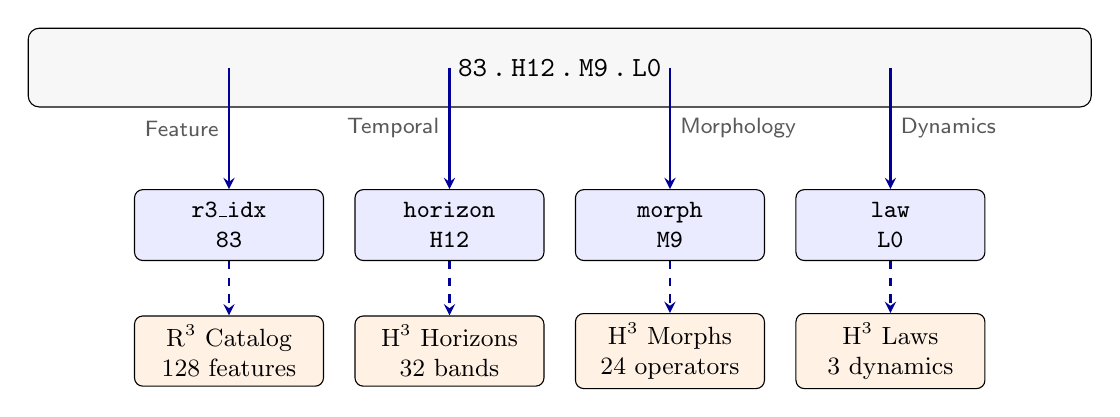
\begin{tikzpicture}[
    comp/.style={
        draw, rounded corners=3pt, fill=blue!8,
        minimum width=2.4cm, minimum height=0.9cm,
        font=\small\ttfamily, align=center
    },
    catalog/.style={
        draw, rounded corners=3pt, fill=orange!10,
        minimum width=2.4cm, minimum height=0.7cm,
        font=\small, align=center
    },
    arr/.style={->, >=stealth, thick, color=blue!60!black},
    lbl/.style={font=\footnotesize\sffamily, color=gray!70!black}
]
    % Full address bar
    \node[draw, rounded corners=4pt, fill=gray!6,
          minimum width=13.5cm, minimum height=1.0cm,
          font=\ttfamily]
        (addr) at (0,0) {83\,.\,H12\,.\,M9\,.\,L0};

    % Invisible anchors for the four segments
    \coordinate (a1) at (-4.2, 0);
    \coordinate (a2) at (-1.4, 0);
    \coordinate (a3) at ( 1.4, 0);
    \coordinate (a4) at ( 4.2, 0);

    % Component boxes below
    \node[comp] (c1) at (-4.2,-2.0) {r3\_idx\\83};
    \node[comp] (c2) at (-1.4,-2.0) {horizon\\H12};
    \node[comp] (c3) at ( 1.4,-2.0) {morph\\M9};
    \node[comp] (c4) at ( 4.2,-2.0) {law\\L0};

    % Arrows from address bar to components
    \draw[arr] (a1) -- (c1) node[midway, left, lbl] {Feature};
    \draw[arr] (a2) -- (c2) node[midway, left, lbl] {Temporal};
    \draw[arr] (a3) -- (c3) node[midway, right, lbl] {Morphology};
    \draw[arr] (a4) -- (c4) node[midway, right, lbl] {Dynamics};

    % Catalog / source layer below components
    \node[catalog] (s1) at (-4.2,-3.6) {R\textsuperscript{3} Catalog\\128 features};
    \node[catalog] (s2) at (-1.4,-3.6) {H\textsuperscript{3} Horizons\\32 bands};
    \node[catalog] (s3) at ( 1.4,-3.6) {H\textsuperscript{3} Morphs\\24 operators};
    \node[catalog] (s4) at ( 4.2,-3.6) {H\textsuperscript{3} Laws\\3 dynamics};

    \draw[arr, dashed] (c1) -- (s1);
    \draw[arr, dashed] (c2) -- (s2);
    \draw[arr, dashed] (c3) -- (s3);
    \draw[arr, dashed] (c4) -- (s4);
\end{tikzpicture}
\caption{Four-tuple spectral address decomposition.
         Each component maps to a specific catalog layer in the
         R\textsuperscript{3}/H\textsuperscript{3} system.}
\label{fig:address-decomposition}
\end{figure}


% ---- Address Construction Rules table ----
\subsection{Address Construction Rules}
\label{subsec:address-rules}

\begin{table}[ht]
\centering
\caption{Address component construction rules.}
\label{tab:address-construction}
\begin{tabular}{@{}llll@{}}
\toprule
\textbf{Component} & \textbf{Source} & \textbf{Range} & \textbf{Example} \\
\midrule
\texttt{r3\_idx} & R\textsuperscript{3} Feature Index & 0--127  & 83  \\
\texttt{horizon} & H\textsuperscript{3} Horizon Index  & H0--H31 & H12 \\
\texttt{morph}   & H\textsuperscript{3} Morph Index    & M0--M23 & M9  \\
\texttt{law}     & H\textsuperscript{3} Law Index      & L0--L2  & L0  \\
\bottomrule
\end{tabular}
\end{table}


% ---- Spectral Label Construction table ----
\subsection{Spectral Label Construction}
\label{subsec:spectral-label}

\begin{table}[ht]
\centering
\caption{Spectral label construction from address components.}
\label{tab:spectral-label}
\begin{tabular}{@{}lll@{}}
\toprule
\textbf{Component} & \textbf{Format} & \textbf{Example} \\
\midrule
Feature    & R\textsuperscript{3} USL name   & \texttt{chroma\_frame\_distance} \\
Horizon    & H\textsuperscript{3} USL label  & \texttt{beat}                   \\
Morph      & H\textsuperscript{3} morph name & \texttt{velocity\_mean}         \\
Law        & H\textsuperscript{3} law name   & \texttt{memory}                 \\
\midrule
Full label & \texttt{feature.horizon.morph.law}
           & \texttt{chroma\_frame\_distance.beat.velocity\_mean.memory} \\
\bottomrule
\end{tabular}
\end{table}


%% ============================================================
%%  SECTION 2 — C³ Unit Interface Table
%% ============================================================
\section{C\textsuperscript{3} Unit Interface Table}
\label{sec:c3-units}

Table~\ref{tab:c3-units} lists all nine C\textsuperscript{3} processing units
and their primary interfaces with the R\textsuperscript{3} feature groups and
H\textsuperscript{3} temporal bands.
R\textsuperscript{3} groups are identified by letter
(A~=~Consonance, B~=~Energy, C~=~Timbre, D~=~Change, E~=~Interactions,
 F~=~Pitch-Class, G~=~Onset Period, H~=~Harmony, I~=~Information,
 J~=~Timbre Ext., K~=~Modulation).
H\textsuperscript{3} bands span Micro ($<$50\,ms), Meso (50\,ms--2\,s),
and Macro ($>$2\,s) perceptual time scales.

\begin{table}[ht]
\centering
\caption{C\textsuperscript{3} unit interface summary.}
\label{tab:c3-units}
\renewcommand{\arraystretch}{1.15}
\begin{tabular}{@{}llclll@{}}
\toprule
\textbf{Unit} & \textbf{Full Name}
  & \textbf{Models}
  & \textbf{Primary R\textsuperscript{3} Groups}
  & \textbf{Primary H\textsuperscript{3} Bands}
  & \textbf{Primary Laws} \\
\midrule
SPU & Sensory Processing    &  9 & A, B, C, D & Micro--Meso  & L0, L2        \\
STU & Structural Timing     & 20 & G, H, I    & Meso--Macro  & L0, L1, L2    \\
IMU & Integrative Memory    & 10 & F, H, I    & Meso--Macro  & L0, L2        \\
ASU & Auditory Scene        &  9 & A, B, C    & Micro--Meso  & L2            \\
NDU & Neuromodulation       &  8 & B, H, I    & Meso--Macro  & L0, L1, L2    \\
MPU & Motor Planning        & 11 & G, H       & Meso         & L0, L1        \\
PCU & Predictive Coding     & 10 & F, H, I    & Micro--Macro & L0, L1, L2    \\
ARU & Arousal Regulation    &  9 & B, H, I    & Meso--Macro  & L0, L1, L2    \\
RPU & Reward Processing     & 10 & H, I, K    & Meso--Macro  & L0, L1, L2    \\
\bottomrule
\end{tabular}
\end{table}


%% ============================================================
%%  SECTION 3 — Provenance Chain Diagram
%% ============================================================
\section{Provenance Chain}
\label{sec:provenance-chain}

Figure~\ref{fig:provenance} traces the complete data-flow from raw audio
to the C\textsuperscript{3} input package.  Every tensor element retains a
spectral address linking it back to its R\textsuperscript{3} source through
an unbroken provenance chain.

\begin{figure}[ht]
\centering
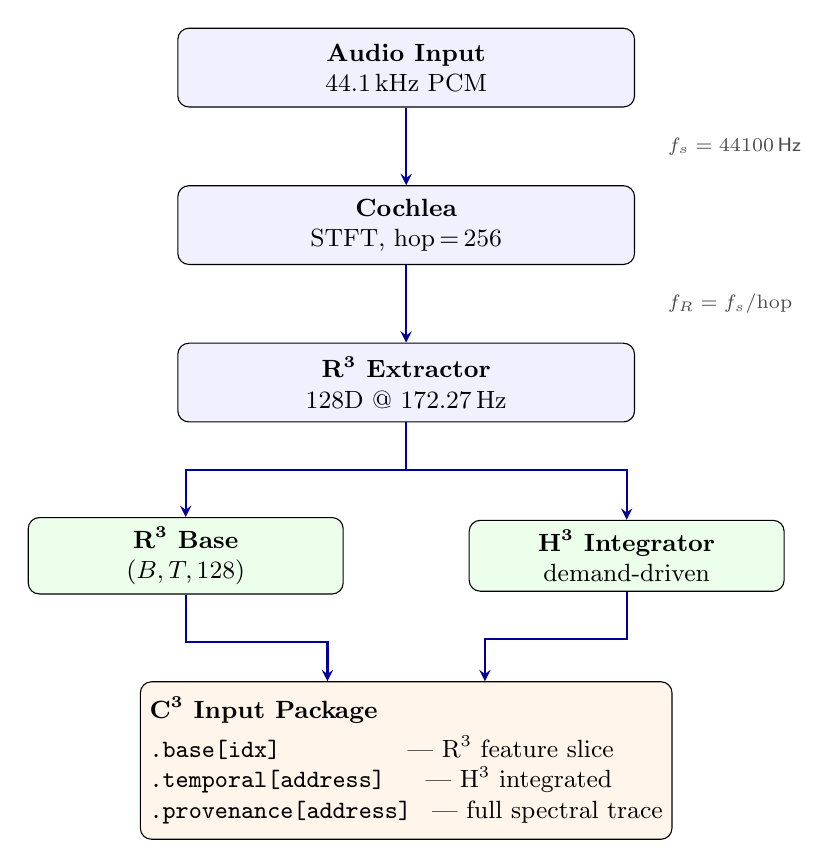
\begin{tikzpicture}[
    block/.style={
        draw, rounded corners=4pt, fill=blue!6,
        minimum width=5.8cm, minimum height=1.0cm,
        font=\small, align=center
    },
    split/.style={
        draw, rounded corners=4pt, fill=green!8,
        minimum width=4.0cm, minimum height=0.9cm,
        font=\small, align=center
    },
    pkg/.style={
        draw, rounded corners=4pt, fill=orange!8,
        minimum width=6.4cm, minimum height=2.0cm,
        font=\small, align=left
    },
    arr/.style={->, >=stealth, thick, color=blue!60!black},
    note/.style={font=\scriptsize\sffamily, color=gray!60!black}
]
    % Top: Audio input
    \node[block] (audio) at (0, 0)
        {\textbf{Audio Input}\\44.1\,kHz PCM};

    % Cochlea
    \node[block] (cochlea) at (0, -2.0)
        {\textbf{Cochlea}\\STFT, hop\,=\,256};
    \draw[arr] (audio) -- (cochlea);
    \node[note, right] at (3.2, -1.0) {$f_s = 44100$\,Hz};

    % R³ Extractor
    \node[block] (r3ext) at (0, -4.0)
        {\textbf{R\textsuperscript{3} Extractor}\\128D @ 172.27\,Hz};
    \draw[arr] (cochlea) -- (r3ext);
    \node[note, right] at (3.2, -3.0) {$f_R = f_s / \mathrm{hop}$};

    % Split into two branches
    \node[split] (r3base) at (-2.8, -6.2)
        {\textbf{R\textsuperscript{3} Base}\\$(B, T, 128)$};
    \node[split] (h3int)  at ( 2.8, -6.2)
        {\textbf{H\textsuperscript{3} Integrator}\\demand-driven};

    \draw[arr] (r3ext.south) -- ++(0,-0.6) -| (r3base.north);
    \draw[arr] (r3ext.south) -- ++(0,-0.6) -| (h3int.north);

    % C³ Input Package
    \node[pkg] (c3pkg) at (0, -8.8)
        {\textbf{C\textsuperscript{3} Input Package}\\[3pt]
         \texttt{.base[idx]}
         \hspace{1.4cm} \textrm{--- R\textsuperscript{3} feature slice}\\
         \texttt{.temporal[address]}
         \hspace{0.3cm} \textrm{--- H\textsuperscript{3} integrated}\\
         \texttt{.provenance[address]}
         \hspace{0.05cm} \textrm{--- full spectral trace}};

    \draw[arr] (r3base.south)  -- ++(0,-0.6) -| ([xshift=-1cm]c3pkg.north);
    \draw[arr] (h3int.south)   -- ++(0,-0.6) -| ([xshift= 1cm]c3pkg.north);
\end{tikzpicture}
\caption{Provenance chain from audio input to C\textsuperscript{3} input package.
         Every tensor element traces back to its R\textsuperscript{3} source
         through spectral addresses.}
\label{fig:provenance}
\end{figure}


%% ============================================================
%%  SECTION 4 — Naming Convention Rules
%% ============================================================
\section{Naming Convention Rules}
\label{sec:naming-rules}

The following rules govern all naming within the Universal Spectral Language.
Violations break the provenance chain and are treated as specification errors.

\begin{enumerate}
    \item \textbf{Measurement, not interpretation.}\enspace
          R\textsuperscript{3} feature names describe what is \emph{measured}
          (e.g.\ \texttt{spectral\_centroid}), never what is
          \emph{perceived} or \emph{interpreted}.

    \item \textbf{No music-theory terms in R\textsuperscript{3}/H\textsuperscript{3}.}\enspace
          Names must not contain \texttt{chord}, \texttt{key},
          \texttt{cadence}, \texttt{tonal}, or \texttt{harmonic}
          in their music-theoretic senses.
          \texttt{harmonic} is permitted only in its signal-processing
          meaning (integer-multiple partials).

    \item \textbf{Perceptual time scales, not musical structure.}\enspace
          H\textsuperscript{3} horizon labels denote perceptual durations.
          For example, \texttt{beat} designates the ${\sim}525$\,ms
          periodicity band, not a musical beat or metrical position.

    \item \textbf{Dot-separated addresses.}\enspace
          Full spectral addresses use dot separation:
          \texttt{feature.horizon.morph.law}.
          No spaces, no slashes, no camelCase.

    \item \textbf{C\textsuperscript{3} music-theory mapping.}\enspace
          C\textsuperscript{3} model documentation \emph{may} reference
          music-theory terms for explanatory purposes, but every such
          reference \emph{must} map to one or more spectral addresses.

    \item \textbf{Unbroken spectral chain.}\enspace
          Every C\textsuperscript{3} input must trace back to an
          R\textsuperscript{3} source through the address system.
          No datum enters C\textsuperscript{3} without a provenance record.
\end{enumerate}
 from main document
% Requires: tikz, booktabs, array, xcolor

%% ============================================================
%%  SECTION 1 — Universal Spectral Address System
%% ============================================================
\section{Universal Spectral Address System}
\label{sec:spectral-address}

Every datum flowing through the MI pipeline carries a \emph{spectral address}:
a four-component tuple that uniquely identifies its origin in the
R\textsuperscript{3}--H\textsuperscript{3} feature--temporal lattice.

\medskip

\begin{center}
\texttt{\{r3\_idx\}.\{horizon\}.\{morph\}.\{law\}}
\end{center}

\medskip

\noindent
\textbf{Numeric example:}\quad \texttt{83.H12.M9.L0}\\[2pt]
\textbf{Spectral label:}\quad
\texttt{chroma\_frame\_distance.beat.velocity\_mean.memory}

% ---- TikZ address decomposition diagram ----
\begin{figure}[ht]
\centering
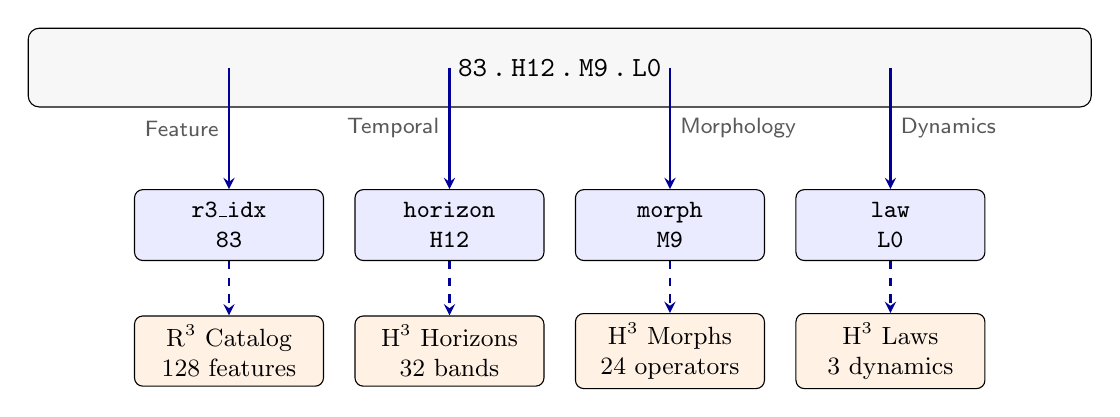
\begin{tikzpicture}[
    comp/.style={
        draw, rounded corners=3pt, fill=blue!8,
        minimum width=2.4cm, minimum height=0.9cm,
        font=\small\ttfamily, align=center
    },
    catalog/.style={
        draw, rounded corners=3pt, fill=orange!10,
        minimum width=2.4cm, minimum height=0.7cm,
        font=\small, align=center
    },
    arr/.style={->, >=stealth, thick, color=blue!60!black},
    lbl/.style={font=\footnotesize\sffamily, color=gray!70!black}
]
    % Full address bar
    \node[draw, rounded corners=4pt, fill=gray!6,
          minimum width=13.5cm, minimum height=1.0cm,
          font=\ttfamily]
        (addr) at (0,0) {83\,.\,H12\,.\,M9\,.\,L0};

    % Invisible anchors for the four segments
    \coordinate (a1) at (-4.2, 0);
    \coordinate (a2) at (-1.4, 0);
    \coordinate (a3) at ( 1.4, 0);
    \coordinate (a4) at ( 4.2, 0);

    % Component boxes below
    \node[comp] (c1) at (-4.2,-2.0) {r3\_idx\\83};
    \node[comp] (c2) at (-1.4,-2.0) {horizon\\H12};
    \node[comp] (c3) at ( 1.4,-2.0) {morph\\M9};
    \node[comp] (c4) at ( 4.2,-2.0) {law\\L0};

    % Arrows from address bar to components
    \draw[arr] (a1) -- (c1) node[midway, left, lbl] {Feature};
    \draw[arr] (a2) -- (c2) node[midway, left, lbl] {Temporal};
    \draw[arr] (a3) -- (c3) node[midway, right, lbl] {Morphology};
    \draw[arr] (a4) -- (c4) node[midway, right, lbl] {Dynamics};

    % Catalog / source layer below components
    \node[catalog] (s1) at (-4.2,-3.6) {R\textsuperscript{3} Catalog\\128 features};
    \node[catalog] (s2) at (-1.4,-3.6) {H\textsuperscript{3} Horizons\\32 bands};
    \node[catalog] (s3) at ( 1.4,-3.6) {H\textsuperscript{3} Morphs\\24 operators};
    \node[catalog] (s4) at ( 4.2,-3.6) {H\textsuperscript{3} Laws\\3 dynamics};

    \draw[arr, dashed] (c1) -- (s1);
    \draw[arr, dashed] (c2) -- (s2);
    \draw[arr, dashed] (c3) -- (s3);
    \draw[arr, dashed] (c4) -- (s4);
\end{tikzpicture}
\caption{Four-tuple spectral address decomposition.
         Each component maps to a specific catalog layer in the
         R\textsuperscript{3}/H\textsuperscript{3} system.}
\label{fig:address-decomposition}
\end{figure}


% ---- Address Construction Rules table ----
\subsection{Address Construction Rules}
\label{subsec:address-rules}

\begin{table}[ht]
\centering
\caption{Address component construction rules.}
\label{tab:address-construction}
\begin{tabular}{@{}llll@{}}
\toprule
\textbf{Component} & \textbf{Source} & \textbf{Range} & \textbf{Example} \\
\midrule
\texttt{r3\_idx} & R\textsuperscript{3} Feature Index & 0--127  & 83  \\
\texttt{horizon} & H\textsuperscript{3} Horizon Index  & H0--H31 & H12 \\
\texttt{morph}   & H\textsuperscript{3} Morph Index    & M0--M23 & M9  \\
\texttt{law}     & H\textsuperscript{3} Law Index      & L0--L2  & L0  \\
\bottomrule
\end{tabular}
\end{table}


% ---- Spectral Label Construction table ----
\subsection{Spectral Label Construction}
\label{subsec:spectral-label}

\begin{table}[ht]
\centering
\caption{Spectral label construction from address components.}
\label{tab:spectral-label}
\begin{tabular}{@{}lll@{}}
\toprule
\textbf{Component} & \textbf{Format} & \textbf{Example} \\
\midrule
Feature    & R\textsuperscript{3} USL name   & \texttt{chroma\_frame\_distance} \\
Horizon    & H\textsuperscript{3} USL label  & \texttt{beat}                   \\
Morph      & H\textsuperscript{3} morph name & \texttt{velocity\_mean}         \\
Law        & H\textsuperscript{3} law name   & \texttt{memory}                 \\
\midrule
Full label & \texttt{feature.horizon.morph.law}
           & \texttt{chroma\_frame\_distance.beat.velocity\_mean.memory} \\
\bottomrule
\end{tabular}
\end{table}


%% ============================================================
%%  SECTION 2 — C³ Unit Interface Table
%% ============================================================
\section{C\textsuperscript{3} Unit Interface Table}
\label{sec:c3-units}

Table~\ref{tab:c3-units} lists all nine C\textsuperscript{3} processing units
and their primary interfaces with the R\textsuperscript{3} feature groups and
H\textsuperscript{3} temporal bands.
R\textsuperscript{3} groups are identified by letter
(A~=~Consonance, B~=~Energy, C~=~Timbre, D~=~Change, E~=~Interactions,
 F~=~Pitch-Class, G~=~Onset Period, H~=~Harmony, I~=~Information,
 J~=~Timbre Ext., K~=~Modulation).
H\textsuperscript{3} bands span Micro ($<$50\,ms), Meso (50\,ms--2\,s),
and Macro ($>$2\,s) perceptual time scales.

\begin{table}[ht]
\centering
\caption{C\textsuperscript{3} unit interface summary.}
\label{tab:c3-units}
\renewcommand{\arraystretch}{1.15}
\begin{tabular}{@{}llclll@{}}
\toprule
\textbf{Unit} & \textbf{Full Name}
  & \textbf{Models}
  & \textbf{Primary R\textsuperscript{3} Groups}
  & \textbf{Primary H\textsuperscript{3} Bands}
  & \textbf{Primary Laws} \\
\midrule
SPU & Sensory Processing    &  9 & A, B, C, D & Micro--Meso  & L0, L2        \\
STU & Structural Timing     & 20 & G, H, I    & Meso--Macro  & L0, L1, L2    \\
IMU & Integrative Memory    & 10 & F, H, I    & Meso--Macro  & L0, L2        \\
ASU & Auditory Scene        &  9 & A, B, C    & Micro--Meso  & L2            \\
NDU & Neuromodulation       &  8 & B, H, I    & Meso--Macro  & L0, L1, L2    \\
MPU & Motor Planning        & 11 & G, H       & Meso         & L0, L1        \\
PCU & Predictive Coding     & 10 & F, H, I    & Micro--Macro & L0, L1, L2    \\
ARU & Arousal Regulation    &  9 & B, H, I    & Meso--Macro  & L0, L1, L2    \\
RPU & Reward Processing     & 10 & H, I, K    & Meso--Macro  & L0, L1, L2    \\
\bottomrule
\end{tabular}
\end{table}


%% ============================================================
%%  SECTION 3 — Provenance Chain Diagram
%% ============================================================
\section{Provenance Chain}
\label{sec:provenance-chain}

Figure~\ref{fig:provenance} traces the complete data-flow from raw audio
to the C\textsuperscript{3} input package.  Every tensor element retains a
spectral address linking it back to its R\textsuperscript{3} source through
an unbroken provenance chain.

\begin{figure}[ht]
\centering
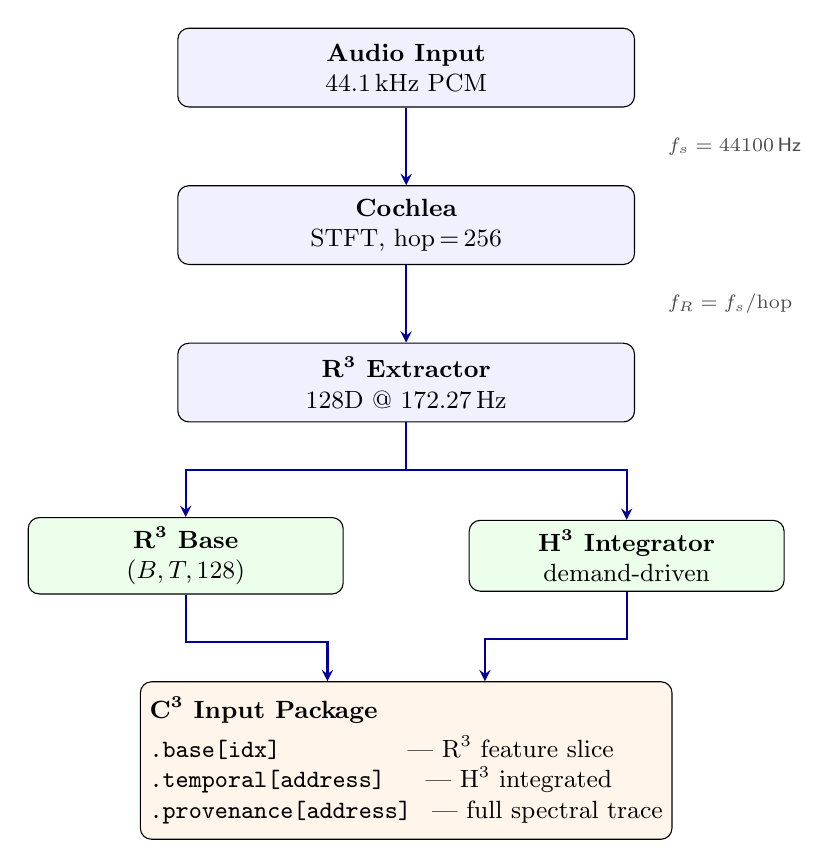
\begin{tikzpicture}[
    block/.style={
        draw, rounded corners=4pt, fill=blue!6,
        minimum width=5.8cm, minimum height=1.0cm,
        font=\small, align=center
    },
    split/.style={
        draw, rounded corners=4pt, fill=green!8,
        minimum width=4.0cm, minimum height=0.9cm,
        font=\small, align=center
    },
    pkg/.style={
        draw, rounded corners=4pt, fill=orange!8,
        minimum width=6.4cm, minimum height=2.0cm,
        font=\small, align=left
    },
    arr/.style={->, >=stealth, thick, color=blue!60!black},
    note/.style={font=\scriptsize\sffamily, color=gray!60!black}
]
    % Top: Audio input
    \node[block] (audio) at (0, 0)
        {\textbf{Audio Input}\\44.1\,kHz PCM};

    % Cochlea
    \node[block] (cochlea) at (0, -2.0)
        {\textbf{Cochlea}\\STFT, hop\,=\,256};
    \draw[arr] (audio) -- (cochlea);
    \node[note, right] at (3.2, -1.0) {$f_s = 44100$\,Hz};

    % R³ Extractor
    \node[block] (r3ext) at (0, -4.0)
        {\textbf{R\textsuperscript{3} Extractor}\\128D @ 172.27\,Hz};
    \draw[arr] (cochlea) -- (r3ext);
    \node[note, right] at (3.2, -3.0) {$f_R = f_s / \mathrm{hop}$};

    % Split into two branches
    \node[split] (r3base) at (-2.8, -6.2)
        {\textbf{R\textsuperscript{3} Base}\\$(B, T, 128)$};
    \node[split] (h3int)  at ( 2.8, -6.2)
        {\textbf{H\textsuperscript{3} Integrator}\\demand-driven};

    \draw[arr] (r3ext.south) -- ++(0,-0.6) -| (r3base.north);
    \draw[arr] (r3ext.south) -- ++(0,-0.6) -| (h3int.north);

    % C³ Input Package
    \node[pkg] (c3pkg) at (0, -8.8)
        {\textbf{C\textsuperscript{3} Input Package}\\[3pt]
         \texttt{.base[idx]}
         \hspace{1.4cm} \textrm{--- R\textsuperscript{3} feature slice}\\
         \texttt{.temporal[address]}
         \hspace{0.3cm} \textrm{--- H\textsuperscript{3} integrated}\\
         \texttt{.provenance[address]}
         \hspace{0.05cm} \textrm{--- full spectral trace}};

    \draw[arr] (r3base.south)  -- ++(0,-0.6) -| ([xshift=-1cm]c3pkg.north);
    \draw[arr] (h3int.south)   -- ++(0,-0.6) -| ([xshift= 1cm]c3pkg.north);
\end{tikzpicture}
\caption{Provenance chain from audio input to C\textsuperscript{3} input package.
         Every tensor element traces back to its R\textsuperscript{3} source
         through spectral addresses.}
\label{fig:provenance}
\end{figure}


%% ============================================================
%%  SECTION 4 — Naming Convention Rules
%% ============================================================
\section{Naming Convention Rules}
\label{sec:naming-rules}

The following rules govern all naming within the Universal Spectral Language.
Violations break the provenance chain and are treated as specification errors.

\begin{enumerate}
    \item \textbf{Measurement, not interpretation.}\enspace
          R\textsuperscript{3} feature names describe what is \emph{measured}
          (e.g.\ \texttt{spectral\_centroid}), never what is
          \emph{perceived} or \emph{interpreted}.

    \item \textbf{No music-theory terms in R\textsuperscript{3}/H\textsuperscript{3}.}\enspace
          Names must not contain \texttt{chord}, \texttt{key},
          \texttt{cadence}, \texttt{tonal}, or \texttt{harmonic}
          in their music-theoretic senses.
          \texttt{harmonic} is permitted only in its signal-processing
          meaning (integer-multiple partials).

    \item \textbf{Perceptual time scales, not musical structure.}\enspace
          H\textsuperscript{3} horizon labels denote perceptual durations.
          For example, \texttt{beat} designates the ${\sim}525$\,ms
          periodicity band, not a musical beat or metrical position.

    \item \textbf{Dot-separated addresses.}\enspace
          Full spectral addresses use dot separation:
          \texttt{feature.horizon.morph.law}.
          No spaces, no slashes, no camelCase.

    \item \textbf{C\textsuperscript{3} music-theory mapping.}\enspace
          C\textsuperscript{3} model documentation \emph{may} reference
          music-theory terms for explanatory purposes, but every such
          reference \emph{must} map to one or more spectral addresses.

    \item \textbf{Unbroken spectral chain.}\enspace
          Every C\textsuperscript{3} input must trace back to an
          R\textsuperscript{3} source through the address system.
          No datum enters C\textsuperscript{3} without a provenance record.
\end{enumerate}


\newpage

% ============================================================================
% SECTION 4: Complete H³ Routing Map
% ============================================================================
%% H³ Routing Map — Complete R³→H³→C³ Data Paths
%% \input{} into main document; no preamble.
%% Extracted from 86 of 96 C³ model documentation files.
%% ARU (10 models) uses qualitative demand specification without explicit tuples.

%% ============================================================
%%  SECTION — Complete Routing Map
%% ============================================================
\section{Complete H\textsuperscript{3} Routing Map}
\label{sec:h3-routing}

This section documents every data path from R\textsuperscript{3} spectral
features through H\textsuperscript{3} temporal morphology to
C\textsuperscript{3} cognitive models.  The routing is
\textbf{asymmetric} (not every feature uses every horizon/morph/law)
but \textbf{deterministic} (each C\textsuperscript{3} model declares
its exact demands).

% ─────────────────────────────────────────────
\subsection{Global Statistics}
\label{subsec:routing-stats}

\begin{table}[H]
\centering
\caption{H\textsuperscript{3} demand overview (extracted from 86 model docs).}
\label{tab:routing-overview}
\renewcommand{\arraystretch}{1.2}
\begin{tabular}{@{}lr@{}}
\toprule
\textbf{Metric} & \textbf{Value} \\
\midrule
Models with explicit demands            & 86 of 96 \\
Models without (ARU, older format)      & 10 \\
Total tuple declarations                & 1{,}737 \\
Unique tuples (global)                  & 746 \\
\quad v1 tuples (R\textsuperscript{3} [0:48])  & 532 \\
\quad v2 tuples (R\textsuperscript{3} [49:127]) & 214 \\
Theoretical space                       & 294{,}912 \\
Active fraction                         & 0.25\% \\
\midrule
R\textsuperscript{3} features used (v1) & 33 of 49 \\
R\textsuperscript{3} features unused    & 16 (all Interaction sub-indices) \\
Horizons used                           & 17 of 32 \\
Morphs used                             & 19 of 24 \\
Laws used                               & 2 of 3 (L0, L2; L1 absent) \\
\bottomrule
\end{tabular}
\end{table}

\paragraph{Notable findings.}
\begin{itemize}\itemsep1pt
  \item \textbf{L1 (prediction) is never used.}
        All 1{,}737 demand tuples use either L0~(memory, 41\%)
        or L2~(integration, 59\%).
        L1 is available in the architecture but no C\textsuperscript{3}
        model currently requests predictive-direction morphology.
  \item \textbf{Interaction sub-indices are sparse.}
        Of the 24 interaction features [25:48], only four are used:
        \texttt{x\_l0l5[0]} (idx~25), \texttt{x\_l4l5[0]} (idx~33),
        \texttt{x\_l4l5[4]} (idx~37, ASU only), and
        \texttt{x\_l5l7[0]} (idx~41).
        The remaining 20 interaction sub-indices are architecturally
        available but currently undemanded.
  \item \textbf{Top~3 features} by demand count:
        \texttt{spectral\_flux}~[10] (157 declarations),
        \texttt{x\_l0l5[0]}~[25] (144),
        \texttt{spectral\_change}~[21] (100).
  \item \textbf{H3 and H16 dominate} horizon usage with 433 and 442
        declarations respectively, reflecting the primacy of
        100\,ms and 1{,}000\,ms integration windows.
\end{itemize}


% ─────────────────────────────────────────────
\subsection{Per-Unit Demand Summary}
\label{subsec:routing-per-unit}

\begin{table}[H]
\centering
\caption{Per-unit H\textsuperscript{3} demand summary.}
\label{tab:unit-demand-summary}
\renewcommand{\arraystretch}{1.15}
\begin{tabular}{@{}lrrrrrrr@{}}
\toprule
\textbf{Unit} & \textbf{Models} & \textbf{Decl.} & \textbf{Unique}
  & \textbf{R\textsuperscript{3} feat.} & \textbf{Horizons}
  & \textbf{Morphs} & \textbf{Laws} \\
\midrule
\rowcolor{grpA!20}
SPU &  9 & 158 & 101 & 25 & 14 & 15 & L0, L2 \\
\rowcolor{grpB!20}
STU & 14 & 298 & 179 & 23 & 13 & 17 & L0, L2 \\
\rowcolor{grpC!20}
IMU & 15 & 347 & 209 & 23 & 15 & 17 & L0, L2 \\
\rowcolor{grpD!20}
ASU &  9 & 158 & 101 & 17 & 12 & 14 & L0, L2 \\
\rowcolor{grpE!20}
NDU &  9 & 181 &  86 & 17 &  8 & 13 & L0, L2 \\
\rowcolor{grpF!20}
MPU & 10 & 177 &  78 & 11 &  9 & 10 & L0, L2 \\
\rowcolor{grpG!20}
PCU & 10 & 215 & 111 & 16 & 10 & 14 & L0, L2 \\
\rowcolor{grpH!20}
ARU & 10 & \multicolumn{6}{c}{\itshape (qualitative demand; explicit tuples pending)} \\
\rowcolor{grpI!20}
RPU & 10 & 203 & 115 & 15 & 10 & 14 & L0, L2 \\
\midrule
\textbf{Total} & \textbf{96} & \textbf{1{,}737} & \textbf{746}
  & \textbf{33} & \textbf{17} & \textbf{19} & \textbf{2} \\
\bottomrule
\end{tabular}
\end{table}


% ─────────────────────────────────────────────
\subsection{Horizon Usage Distribution}
\label{subsec:routing-horizons}

\begin{figure}[H]
\centering
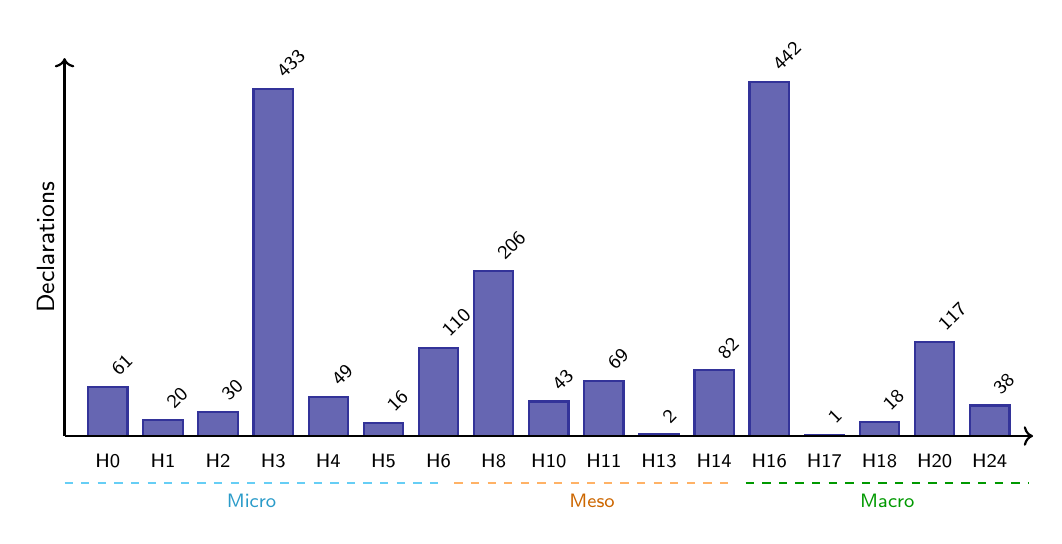
\begin{tikzpicture}[
  bar/.style={fill=NavyBlue!60, draw=NavyBlue!80, thick},
  lbl/.style={font=\scriptsize\sffamily, rotate=45, anchor=west}
]
  % Data: H0:61, H1:20, H2:30, H3:433, H4:49, H5:16, H6:110,
  %        H8:206, H10:43, H11:69, H13:2, H14:82, H16:442,
  %        H17:1, H18:18, H20:117, H24:38
  % Scale: max=442, bar width=0.55cm, height factor=4.5/442
  \def\hf{0.01018}  % 4.5/442
  \foreach \h/\v/\x in {
    H0/61/0, H1/20/0.7, H2/30/1.4, H3/433/2.1, H4/49/2.8,
    H5/16/3.5, H6/110/4.2, H8/206/4.9, H10/43/5.6,
    H11/69/6.3, H13/2/7.0, H14/82/7.7, H16/442/8.4,
    H17/1/9.1, H18/18/9.8, H20/117/10.5, H24/38/11.2
  }{
    \draw[bar] (\x, 0) rectangle (\x+0.5, \v*\hf);
    \node[lbl] at (\x+0.25, \v*\hf+0.1) {\v};
    \node[font=\scriptsize\sffamily, below] at (\x+0.25, -0.1) {\h};
  }
  % Bands
  \draw[thick, cyan!60, dashed] (-0.3, -0.6) -- (4.45, -0.6)
    node[midway, below, font=\scriptsize\sffamily, cyan!80!black] {Micro};
  \draw[thick, orange!60, dashed] (4.65, -0.6) -- (8.15, -0.6)
    node[midway, below, font=\scriptsize\sffamily, orange!80!black] {Meso};
  \draw[thick, green!60!black, dashed] (8.35, -0.6) -- (11.95, -0.6)
    node[midway, below, font=\scriptsize\sffamily, green!60!black] {Macro};
  % Axis
  \draw[->, thick] (-0.3, 0) -- (12.0, 0);
  \draw[->, thick] (-0.3, 0) -- (-0.3, 4.8)
    node[midway, rotate=90, above, font=\small\sffamily] {Declarations};
\end{tikzpicture}
\caption{H\textsuperscript{3} horizon usage across all 86 models.
H3 (100\,ms) and H16 (1{,}s) dominate, reflecting the two primary
temporal scales of auditory cognition.}
\label{fig:horizon-usage}
\end{figure}


% ─────────────────────────────────────────────
\subsection{Morph Usage Distribution}
\label{subsec:routing-morphs}

\begin{table}[H]
\centering
\caption{Morph usage frequency across all 86 models.
Five morphs (M7, M9, M10, M12, M23) are architecturally defined
but currently undemanded by any C\textsuperscript{3} model.}
\label{tab:morph-usage}
\renewcommand{\arraystretch}{1.1}
\begin{tabular}{@{}rlrrp{5.5cm}@{}}
\toprule
\textbf{Morph} & \textbf{Name} & \textbf{Count} & \textbf{\%} & \textbf{Category} \\
\midrule
\rowcolor{cyan!8}
M0  & \texttt{attn\_mean}   & 689 & 39.7 & Distribution \\
\rowcolor{cyan!8}
M1  & \texttt{mean}         & 428 & 24.6 & Distribution \\
\rowcolor{green!8}
M14 & \texttt{periodicity}  & 146 &  8.4 & Rhythm \\
\rowcolor{orange!8}
M8  & \texttt{velocity}     &  93 &  5.4 & Dynamics \\
\rowcolor{orange!8}
M18 & \texttt{trend}        &  82 &  5.1 & Dynamics \\
\rowcolor{cyan!8}
M2  & \texttt{std}          &  71 &  4.1 & Distribution \\
\rowcolor{magenta!8}
M20 & \texttt{entropy}      &  58 &  3.3 & Information \\
\rowcolor{cyan!8}
M3  & \texttt{median}       &  26 &  1.5 & Distribution \\
\rowcolor{cyan!8}
M4  & \texttt{max}          &  27 &  1.6 & Distribution \\
\rowcolor{green!8}
M17 & \texttt{shape\_period} & 25 &  1.4 & Rhythm \\
\rowcolor{blue!8}
M19 & \texttt{stability}    &  36 &  2.1 & Geometry \\
\rowcolor{orange!8}
M15 & \texttt{smoothness}   &  12 &  0.7 & Dynamics \\
\rowcolor{orange!8}
M13 & \texttt{accel\_std}   &  12 &  0.7 & Dynamics \\
\rowcolor{green!8}
M22 & \texttt{peaks}        &  11 &  0.6 & Rhythm \\
\rowcolor{orange!8}
M21 & \texttt{zero\_cross}  &   8 &  0.5 & Dynamics \\
\rowcolor{cyan!8}
M5  & \texttt{range}        &   6 &  0.3 & Distribution \\
\rowcolor{cyan!8}
M6  & \texttt{skewness}     &   3 &  0.2 & Distribution \\
\rowcolor{orange!8}
M11 & \texttt{acceleration} &   2 &  0.1 & Dynamics \\
\rowcolor{blue!8}
M16 & \texttt{curvature}    &   2 &  0.1 & Geometry \\
\midrule
\multicolumn{5}{l}{\itshape Unused morphs: M7 (kurtosis), M9 (velocity\_mean),
M10 (velocity\_std), M12 (accel\_mean), M23 (symmetry)} \\
\bottomrule
\end{tabular}
\end{table}


% ─────────────────────────────────────────────
\subsection{Law Usage}
\label{subsec:routing-laws}

\begin{table}[H]
\centering
\caption{H\textsuperscript{3} law usage across all 86 models.}
\label{tab:law-usage}
\renewcommand{\arraystretch}{1.15}
\begin{tabular}{@{}rlrrl@{}}
\toprule
\textbf{Law} & \textbf{Name} & \textbf{Count} & \textbf{\%} & \textbf{Status} \\
\midrule
L0 & Memory (past $\to$ present)               & 713  & 41.0 & Active \\
L1 & Prediction (present $\to$ future)          &   0  &  0.0 & \textbf{Unused} \\
L2 & Integration (past $\leftrightarrow$ future) & 1{,}024 & 59.0 & Active \\
\bottomrule
\end{tabular}
\end{table}

\noindent
\textbf{Why is L1 absent?}\quad
L1 (prediction) requires future frames, introducing latency equal
to the horizon duration.
All 86 models with explicit demands chose either causal (L0) or
bidirectional (L2) windowing.
L1 remains architecturally available for models that explicitly
require predictive-only temporal perspective.


% ─────────────────────────────────────────────
\subsection{R\textsuperscript{3} Feature Routing Table (v1, [0:48])}
\label{subsec:routing-r3-table}

Table~\ref{tab:r3-routing} shows the complete routing for each v1
R\textsuperscript{3} feature: which horizons, morphs, laws, and
C\textsuperscript{3} units consume it.

{\small
\renewcommand{\arraystretch}{1.05}
\begin{longtable}{@{}
  r
  >{\raggedright}p{2.1cm}
  c
  >{\raggedright}p{3.5cm}
  c
  >{\raggedright}p{3.0cm}
  c
  >{\raggedright\arraybackslash}p{2.8cm}
@{}}
\caption{Complete R\textsuperscript{3} $\to$ H\textsuperscript{3} routing
for all v1 features.  ``\#H'' = number of distinct horizons used;
``Units'' = C\textsuperscript{3} units that demand this feature
through H\textsuperscript{3}.}
\label{tab:r3-routing} \\
\toprule
\textbf{Idx} & \textbf{Feature} & \textbf{\#H} & \textbf{Horizons}
  & \textbf{\#M} & \textbf{Morphs} & \textbf{Laws}
  & \textbf{Units} \\
\midrule
\endfirsthead
\toprule
\textbf{Idx} & \textbf{Feature} & \textbf{\#H} & \textbf{Horizons}
  & \textbf{\#M} & \textbf{Morphs} & \textbf{Laws}
  & \textbf{Units} \\
\midrule
\endhead
\midrule
\multicolumn{8}{r}{\footnotesize\itshape continued on next page} \\
\endfoot
\bottomrule
\endlastfoot

%% ── Group A: Consonance [0:6] ──
\rowcolor{grpA}
0  & roughness        & 10 & H0,3,6,8,10,14, 16,18,20,24
   & 8  & M0,1,2,6,8, 14,18,20 & L0,L2
   & SPU,STU,IMU, ASU,NDU,PCU, RPU \\
\rowcolor{grpA}
1  & sethares\_diss.  &  7 & H0,3,8,10,14, 16,24
   & 4  & M0,1,8,19 & L0,L2
   & ASU,IMU,SPU \\
\rowcolor{grpA}
2  & helmholtz\_kang  &  5 & H0,3,6,8,18
   & 3  & M0,1,19 & L0,L2
   & IMU,SPU,STU \\
\rowcolor{grpA}
3  & stumpf\_fusion   &  9 & H0,3,6,10,14, 16,18,20,24
   & 7  & M0,1,3,6,8,14,19 & L0,L2
   & ASU,IMU,MPU, SPU \\
\rowcolor{grpA}
4  & sensory\_pleas.  &  7 & H3,8,10,16,18, 20,24
   & 8  & M0,1,2,8,15, 18,19,20 & L0,L2
   & ASU,IMU,NDU, PCU,RPU,SPU \\
\rowcolor{grpA}
5  & inharmonicity    & 12 & H0,1,3,5,6,8, 10,11,14,16,20,24
   & 8  & M0,1,2,8,14, 18,19,22 & L0,L2
   & ASU,IMU,PCU, SPU \\
\rowcolor{grpA}
6  & harmonic\_dev.   &  6 & H0,3,10,14,16,20
   & 3  & M0,1,4 & L0,L2
   & IMU,PCU,SPU \\

%% ── Group B: Energy [7:11] ──
\rowcolor{grpB}
7  & amplitude        & 10 & H0,1,3,6,8,11, 14,16,20,24
   & 10 & M0,1,2,3,4,5, 8,15,18,20 & L0,L2
   & ASU,IMU,MPU, NDU,PCU,RPU, STU \\
\rowcolor{grpB}
8  & loudness         &  7 & H3,6,8,11,14, 16,20
   & 12 & M0,1,2,4,5,8, 14,15,17,18, 19,20 & L0,L2
   & \textit{all 8 units} \\
\rowcolor{grpB}
9  & acceleration\_A  &  6 & H3,4,8,11,14,16
   & 5  & M0,1,8,14,15 & L0,L2
   & ASU,PCU,RPU, STU \\
\rowcolor{grpB}
10 & spectral\_flux   & 11 & H0,1,3,4,6,8, 10,11,16,20,24
   & 9  & M0,1,2,3,4,8, 14,17,19 & L0,L2
   & \textit{all 8 units} \\
\rowcolor{grpB}
11 & onset\_strength  & 10 & H0,3,6,8,10,11, 13,14,16,20
   & 10 & M0,1,2,4,5,8, 11,14,15,17 & L0,L2
   & ASU,IMU,MPU, NDU,PCU,SPU, STU \\

%% ── Group C: Timbre [12:20] ──
\rowcolor{grpC}
12 & warmth           &  8 & H2,3,5,8,14, 16,20,24
   & 4  & M0,1,3,19 & L0,L2
   & IMU,MPU,RPU, SPU,STU \\
\rowcolor{grpC}
13 & sharpness        &  4 & H2,3,4,16
   & 6  & M0,1,2,8,17,20 & L0,L2
   & NDU,RPU,SPU, STU \\
\rowcolor{grpC}
14 & tonalness        & 13 & H0,1,2,3,4,5,6, 8,10,14,16,20,24
   & 8  & M0,1,2,3,14, 18,19,22 & L0,L2
   & ASU,IMU,NDU, PCU,RPU,SPU, STU \\
\rowcolor{grpC}
15 & clarity          &  5 & H3,5,8,10,18
   & 4  & M0,1,2,3 & L0,L2
   & ASU,IMU,MPU, SPU,STU \\
\rowcolor{grpC}
16 & spec.\_smooth.   &  5 & H0,3,14,16,20
   & 4  & M0,1,2,20 & L0,L2
   & ASU,IMU,NDU, SPU,STU \\
\rowcolor{grpC}
17 & spec.\_autocorr. &  4 & H3,6,8,10
   & 3  & M0,1,14 & L0,L2
   & IMU,NDU,SPU, STU \\
\rowcolor{grpC}
18 & tristimulus1     &  7 & H0,2,3,6,16,20,24
   & 3  & M0,1,22 & L0,L2
   & IMU,SPU,STU \\
\rowcolor{grpC}
19 & tristimulus2     &  3 & H0,2,3
   & 1  & M0 & L2
   & SPU,STU \\
\rowcolor{grpC}
20 & tristimulus3     &  3 & H0,2,3
   & 1  & M0 & L2
   & SPU,STU \\

%% ── Group D: Change [21:24] ──
\rowcolor{grpD}
21 & spectral\_change & 11 & H1,2,3,4,8,10, 11,14,16,18,20
   & 14 & M0,1,2,3,4,5, 8,13,14,15,17, 18,19,20 & L0,L2
   & \textit{all 8 units} \\
\rowcolor{grpD}
22 & energy\_change   & 11 & H3,4,6,8,10,11, 14,16,18,20,24
   & 12 & M0,1,2,3,8,11, 13,14,15,18, 19,20 & L0,L2
   & \textit{all 8 units} \\
\rowcolor{grpD}
23 & pitch\_change    &  9 & H3,4,6,8,11, 14,16,20,24
   & 9  & M0,1,2,3,8, 14,18,19,20 & L0,L2
   & IMU,NDU,PCU, SPU,STU \\
\rowcolor{grpD}
24 & concentration    &  5 & H3,4,8,14,16
   & 6  & M0,1,2,3,19,20 & L0,L2
   & NDU,RPU,SPU, STU \\

%% ── Group E: Interactions [25:48] ──
\rowcolor{grpE}
25 & x\_l0l5[0]       & 11 & H0,1,3,4,6,8, 11,14,16,17,20
   & 14 & M0,1,2,8,13, 14,15,16,17,18, 19,20,21,22 & L0,L2
   & \textit{all 8 units} \\
\rowcolor{grpE}
33 & x\_l4l5[0]       &  7 & H3,4,8,11,14,16,20
   & 10 & M0,1,2,8,14, 17,18,19,20,22 & L0,L2
   & IMU,MPU,NDU, PCU,RPU,SPU, STU \\
\rowcolor{grpE}
37 & x\_l4l5[4]       &  2 & H3,16
   & 6  & M0,1,2,17,20,21 & L2
   & ASU \\
\rowcolor{grpE}
41 & x\_l5l7[0]       &  6 & H3,6,8,14,16,20
   & 11 & M0,1,2,5,6,13, 14,16,18,19,20 & L0,L2
   & IMU,NDU,PCU, RPU,SPU,STU \\[3pt]
\multicolumn{8}{l}{\footnotesize\itshape
  Indices 26--32, 34--36, 38--40, 42--48 are architecturally defined
  but undemanded by any model.} \\

\end{longtable}
}% end \small


% ─────────────────────────────────────────────
\subsection{Unit--Feature Affinity Matrix}
\label{subsec:routing-affinity}

Figure~\ref{fig:unit-feature-affinity} shows which R\textsuperscript{3}
feature groups are consumed by each C\textsuperscript{3} unit through
H\textsuperscript{3}.  Cell shading intensity reflects the number of
unique demand tuples.

\begin{figure}[H]
\centering
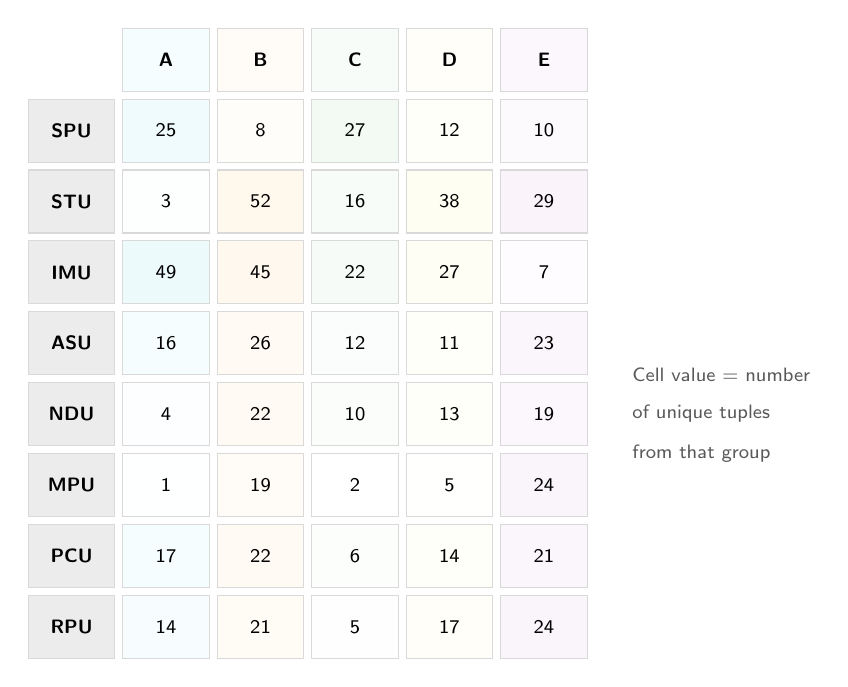
\begin{tikzpicture}[
  cell/.style={minimum width=1.1cm, minimum height=0.8cm,
    font=\scriptsize\sffamily, align=center, draw=gray!30},
  header/.style={cell, font=\scriptsize\sffamily\bfseries,
    fill=gray!15},
  scale=1.0
]
  % Column headers (R³ groups)
  \foreach \g/\x/\c in {
    A/1/grpA, B/2/grpB, C/3/grpC, D/4/grpD, E/5/grpE%
  }{
    \node[header, fill=\c!30] at (\x*1.2, 0) {\g};
  }

  % Row headers (Units) and data
  % SPU: A=25, B=8, C=27, D=12, E=10
  \node[header] at (0, -0.9) {SPU};
  \node[cell, fill=grpA!50] at (1.2, -0.9) {25};
  \node[cell, fill=grpB!15] at (2.4, -0.9) {8};
  \node[cell, fill=grpC!55] at (3.6, -0.9) {27};
  \node[cell, fill=grpD!25] at (4.8, -0.9) {12};
  \node[cell, fill=grpE!20] at (6.0, -0.9) {10};

  % STU: A=3, B=52, C=16, D=38, E=29
  \node[header] at (0, -1.8) {STU};
  \node[cell, fill=grpA!5] at (1.2, -1.8) {3};
  \node[cell, fill=grpB!60] at (2.4, -1.8) {52};
  \node[cell, fill=grpC!30] at (3.6, -1.8) {16};
  \node[cell, fill=grpD!50] at (4.8, -1.8) {38};
  \node[cell, fill=grpE!45] at (6.0, -1.8) {29};

  % IMU: A=49, B=45, C=22, D=27, E=7
  \node[header] at (0, -2.7) {IMU};
  \node[cell, fill=grpA!60] at (1.2, -2.7) {49};
  \node[cell, fill=grpB!55] at (2.4, -2.7) {45};
  \node[cell, fill=grpC!35] at (3.6, -2.7) {22};
  \node[cell, fill=grpD!40] at (4.8, -2.7) {27};
  \node[cell, fill=grpE!10] at (6.0, -2.7) {7};

  % ASU: A=16, B=26, C=12, D=11, E=23
  \node[header] at (0, -3.6) {ASU};
  \node[cell, fill=grpA!30] at (1.2, -3.6) {16};
  \node[cell, fill=grpB!40] at (2.4, -3.6) {26};
  \node[cell, fill=grpC!20] at (3.6, -3.6) {12};
  \node[cell, fill=grpD!20] at (4.8, -3.6) {11};
  \node[cell, fill=grpE!35] at (6.0, -3.6) {23};

  % NDU: A=4, B=22, C=10, D=13, E=19
  \node[header] at (0, -4.5) {NDU};
  \node[cell, fill=grpA!8] at (1.2, -4.5) {4};
  \node[cell, fill=grpB!35] at (2.4, -4.5) {22};
  \node[cell, fill=grpC!18] at (3.6, -4.5) {10};
  \node[cell, fill=grpD!25] at (4.8, -4.5) {13};
  \node[cell, fill=grpE!30] at (6.0, -4.5) {19};

  % MPU: A=1, B=19, C=2, D=5, E=24
  \node[header] at (0, -5.4) {MPU};
  \node[cell, fill=grpA!3] at (1.2, -5.4) {1};
  \node[cell, fill=grpB!30] at (2.4, -5.4) {19};
  \node[cell, fill=grpC!5] at (3.6, -5.4) {2};
  \node[cell, fill=grpD!10] at (4.8, -5.4) {5};
  \node[cell, fill=grpE!38] at (6.0, -5.4) {24};

  % PCU: A=17, B=22, C=6, D=14, E=21
  \node[header] at (0, -6.3) {PCU};
  \node[cell, fill=grpA!30] at (1.2, -6.3) {17};
  \node[cell, fill=grpB!35] at (2.4, -6.3) {22};
  \node[cell, fill=grpC!12] at (3.6, -6.3) {6};
  \node[cell, fill=grpD!25] at (4.8, -6.3) {14};
  \node[cell, fill=grpE!33] at (6.0, -6.3) {21};

  % RPU: A=14, B=21, C=5, D=17, E=24
  \node[header] at (0, -7.2) {RPU};
  \node[cell, fill=grpA!25] at (1.2, -7.2) {14};
  \node[cell, fill=grpB!33] at (2.4, -7.2) {21};
  \node[cell, fill=grpC!10] at (3.6, -7.2) {5};
  \node[cell, fill=grpD!28] at (4.8, -7.2) {17};
  \node[cell, fill=grpE!38] at (6.0, -7.2) {24};

  % Legend
  \node[font=\scriptsize\sffamily, text=gray!70!black, anchor=west]
    at (7.0, -4.0) {Cell value = number};
  \node[font=\scriptsize\sffamily, text=gray!70!black, anchor=west]
    at (7.0, -4.5) {of unique tuples};
  \node[font=\scriptsize\sffamily, text=gray!70!black, anchor=west]
    at (7.0, -5.0) {from that group};
\end{tikzpicture}
\caption{Unit--feature group affinity matrix.
Cell values show the number of unique H\textsuperscript{3} demand tuples
from each R\textsuperscript{3} group per unit.
Darker shading = higher demand density.}
\label{fig:unit-feature-affinity}
\end{figure}


% ─────────────────────────────────────────────
\subsection{Per-Unit Detailed Routing}
\label{subsec:routing-per-unit-detail}

The following tables show every R\textsuperscript{3} feature consumed by
each unit through H\textsuperscript{3}, including exact horizon, morph,
and law ranges.

%% ── SPU ──
\subsubsection*{SPU --- Sensory Processing Unit (9 models, 71 v1 tuples)}

{\footnotesize
\begin{longtable}{@{}r l r l l l@{}}
\toprule
\textbf{R\textsuperscript{3}} & \textbf{Feature} & \textbf{\#}
  & \textbf{Horizons} & \textbf{Morphs} & \textbf{Laws} \\
\midrule
\endfirsthead
\midrule
\endhead
\endfoot
\bottomrule
\endlastfoot

\rowcolor{grpA}
0 & roughness & 5 & H0,3,6 & M0,1,14,18 & L0,L2 \\
\rowcolor{grpA}
1 & sethares\_diss. & 1 & H0 & M0 & L2 \\
\rowcolor{grpA}
2 & helmholtz\_kang & 4 & H0,3,6 & M0,1,19 & L0,L2 \\
\rowcolor{grpA}
3 & stumpf\_fusion & 2 & H0,6 & M0,1 & L0,L2 \\
\rowcolor{grpA}
4 & sensory\_pleas. & 1 & H3 & M0 & L2 \\
\rowcolor{grpA}
5 & inharmonicity & 6 & H0,3,5,6 & M0,1,18 & L0,L2 \\
\rowcolor{grpA}
6 & harmonic\_dev. & 2 & H0,3 & M0,1 & L0,L2 \\
\rowcolor{grpB}
8 & loudness & 1 & H8 & M1 & L0 \\
\rowcolor{grpB}
11 & onset\_str. & 1 & H3 & M0 & L0 \\
\rowcolor{grpC}
12 & warmth & 2 & H2,5 & M0,1 & L0,L2 \\
\rowcolor{grpC}
13 & sharpness & 1 & H2 & M0 & L2 \\
\rowcolor{grpC}
14 & tonalness & 7 & H0,2,3,5,6,8 & M0,1,19 & L0,L2 \\
\rowcolor{grpC}
15 & clarity & 2 & H3,8 & M0,1 & L0,L2 \\
\rowcolor{grpC}
16 & spec.~smooth. & 1 & H3 & M0 & L2 \\
\rowcolor{grpC}
17 & spec.~autocorr. & 3 & H3,6 & M0,14 & L2 \\
\rowcolor{grpC}
18 & tristimulus1 & 4 & H0,2,3,6 & M0,1 & L0,L2 \\
\rowcolor{grpC}
19 & tristimulus2 & 3 & H0,2,3 & M0 & L2 \\
\rowcolor{grpC}
20 & tristimulus3 & 3 & H0,2,3 & M0 & L2 \\
\rowcolor{grpD}
21 & spec.~change & 3 & H3,8 & M1,8,13 & L0 \\
\rowcolor{grpD}
22 & energy\_change & 3 & H3,6,8 & M0,1,8 & L0,L2 \\
\rowcolor{grpD}
23 & pitch\_change & 3 & H3,6 & M0,1,8 & L0,L2 \\
\rowcolor{grpD}
24 & concentration & 3 & H3,8 & M0,1,3 & L0,L2 \\
\rowcolor{grpE}
25 & x\_l0l5[0] & 2 & H3,6 & M0,14 & L2 \\
\rowcolor{grpE}
33 & x\_l4l5[0] & 2 & H8 & M0,14 & L2 \\
\rowcolor{grpE}
41 & x\_l5l7[0] & 6 & H3,6,8 & M0,1,14,19 & L0,L2 \\
\end{longtable}
}


%% ── STU ──
\subsubsection*{STU --- Structural Timing Unit (14 models, 140 v1 tuples)}

{\footnotesize
\begin{longtable}{@{}r l r l l l@{}}
\toprule
\textbf{R\textsuperscript{3}} & \textbf{Feature} & \textbf{\#}
  & \textbf{Horizons} & \textbf{Morphs} & \textbf{Laws} \\
\midrule
\endfirsthead
\midrule
\endhead
\endfoot
\bottomrule
\endlastfoot

\rowcolor{grpA}
0 & roughness & 2 & H20 & M1,18 & L0 \\
\rowcolor{grpA}
2 & helmholtz\_kang & 1 & H8 & M1 & L0 \\
\rowcolor{grpB}
7 & amplitude & 13 & H6,8,11,14,16,20 & M0,1,3,4,15,18 & L0,L2 \\
\rowcolor{grpB}
8 & loudness & 15 & H6,11,14,16,20 & M0,1,4,14,15,18,19 & L0 \\
\rowcolor{grpB}
9 & accel.~A & 5 & H8,11,14,16 & M0,1,14,15 & L0,L2 \\
\rowcolor{grpB}
10 & spec.~flux & 11 & H6,8,11,16 & M0,1,4,8,14,17 & L0 \\
\rowcolor{grpB}
11 & onset\_str. & 9 & H6,8,11,16 & M0,1,4,14,15,17 & L0 \\
\rowcolor{grpC}
12 & warmth & 3 & H2,14 & M0,1,3 & L0,L2 \\
\rowcolor{grpC}
13 & sharpness & 1 & H2 & M0 & L2 \\
\rowcolor{grpC}
14 & tonalness & 7 & H5,6,8,14 & M0,1,3 & L0,L2 \\
\rowcolor{grpC}
15 & clarity & 1 & H5 & M0 & L0 \\
\rowcolor{grpC}
16 & spec.~smooth. & 1 & H14 & M1 & L0 \\
\rowcolor{grpC}
17 & spec.~autocorr. & 2 & H8 & M0,1 & L0,L2 \\
\rowcolor{grpC}
18 & tristimulus1 & 3 & H2,20 & M0,1,22 & L0,L2 \\
\rowcolor{grpC}
19 & tristimulus2 & 1 & H2 & M0 & L2 \\
\rowcolor{grpC}
20 & tristimulus3 & 1 & H2 & M0 & L2 \\
\rowcolor{grpD}
21 & spec.~change & 9 & H8,11,16 & M1,3,8,14,15,17 & L0,L2 \\
\rowcolor{grpD}
22 & energy\_change & 13 & H6,8,11,14,16 & M1,3,8,11,13,14,15 & L0,L2 \\
\rowcolor{grpD}
23 & pitch\_change & 8 & H8,14,16,20 & M0,1,3,8,14,18 & L0,L2 \\
\rowcolor{grpD}
24 & concentration & 5 & H8,14,16 & M0,1,3,19 & L0 \\
\rowcolor{grpE}
25 & x\_l0l5[0] & 12 & H11,14,16,20 & M0,1,13,14,15,19,22 & L0,L2 \\
\rowcolor{grpE}
33 & x\_l4l5[0] & 10 & H11,14,16,20 & M0,1,14,17,18,19,22 & L0,L2 \\
\rowcolor{grpE}
41 & x\_l5l7[0] & 7 & H14,16,20 & M1,13,14,18,19 & L0,L2 \\
\end{longtable}
}


%% ── IMU ──
\subsubsection*{IMU --- Integrative Memory Unit (15 models, 150 v1 tuples)}

{\footnotesize
\begin{longtable}{@{}r l r l l l@{}}
\toprule
\textbf{R\textsuperscript{3}} & \textbf{Feature} & \textbf{\#}
  & \textbf{Horizons} & \textbf{Morphs} & \textbf{Laws} \\
\midrule
\endfirsthead
\midrule
\endhead
\endfoot
\bottomrule
\endlastfoot

\rowcolor{grpA}
0 & roughness & 7 & H10,14,16,18,20,24 & M0,1,18 & L0,L2 \\
\rowcolor{grpA}
1 & sethares\_diss. & 4 & H10,14,16,24 & M0,1,8,19 & L0,L2 \\
\rowcolor{grpA}
2 & helmholtz\_kang & 1 & H18 & M1 & L0 \\
\rowcolor{grpA}
3 & stumpf\_fusion & 16 & H0,3,6,10,14,16,18,20,24 & M0,1,3,14,19 & L0,L2 \\
\rowcolor{grpA}
4 & sensory\_pleas. & 7 & H10,16,18,20,24 & M0,1,18,19 & L0,L2 \\
\rowcolor{grpA}
5 & inharmonicity & 10 & H6,10,11,14,16,20,24 & M0,1,8,14,19,22 & L0,L2 \\
\rowcolor{grpA}
6 & harmonic\_dev. & 4 & H10,14,16,20 & M0,1 & L0,L2 \\
\rowcolor{grpB}
7 & amplitude & 13 & H6,11,16,20,24 & M0,1,3,4,5,8,18 & L0,L2 \\
\rowcolor{grpB}
8 & loudness & 5 & H6,11,16 & M0,1,8,17 & L0,L2 \\
\rowcolor{grpB}
10 & spec.~flux & 13 & H6,10,11,16,20,24 & M0,1,3,4,14,17,19 & L0,L2 \\
\rowcolor{grpB}
11 & onset\_str. & 14 & H6,10,11,14,16,20 & M0,1,4,5,8,14,17 & L0,L2 \\
\rowcolor{grpC}
12 & warmth & 3 & H16,20,24 & M0,1,19 & L0,L2 \\
\rowcolor{grpC}
14 & tonalness & 11 & H0,3,6,10,14,16,20,24 & M0,1,3,18,19,22 & L0,L2 \\
\rowcolor{grpC}
15 & clarity & 2 & H10,18 & M0,3 & L0,L2 \\
\rowcolor{grpC}
16 & spec.~smooth. & 1 & H20 & M1 & L0 \\
\rowcolor{grpC}
17 & spec.~autocorr. & 3 & H3,6,10 & M14 & L0,L2 \\
\rowcolor{grpC}
18 & tristimulus1 & 2 & H16,24 & M0,1 & L0,L2 \\
\rowcolor{grpD}
21 & spec.~change & 9 & H10,14,16,18,20 & M0,1,3,4,5,8 & L0,L2 \\
\rowcolor{grpD}
22 & energy\_change & 13 & H6,10,11,14,16,18,20,24 & M0,1,13,14,18,19 & L0,L2 \\
\rowcolor{grpD}
23 & pitch\_change & 5 & H11,14,16,20,24 & M0,1,19 & L0,L2 \\
\rowcolor{grpE}
25 & x\_l0l5[0] & 2 & H6,16 & M0,19 & L0,L2 \\
\rowcolor{grpE}
33 & x\_l4l5[0] & 2 & H11 & M0,17 & L0,L2 \\
\rowcolor{grpE}
41 & x\_l5l7[0] & 3 & H16 & M1,14,18 & L0,L2 \\
\end{longtable}
}


%% ── ASU ──
\subsubsection*{ASU --- Auditory Scene Analysis Unit (9 models, 87 v1 tuples)}

{\footnotesize
\begin{longtable}{@{}r l r l l l@{}}
\toprule
\textbf{R\textsuperscript{3}} & \textbf{Feature} & \textbf{\#}
  & \textbf{Horizons} & \textbf{Morphs} & \textbf{Laws} \\
\midrule
\endfirsthead
\midrule
\endhead
\endfoot
\bottomrule
\endlastfoot

\rowcolor{grpA}
0 & roughness & 6 & H0,3,16 & M0,1,2,20 & L2 \\
\rowcolor{grpA}
1 & sethares\_diss. & 2 & H3,8 & M0,8 & L0,L2 \\
\rowcolor{grpA}
3 & stumpf\_fusion & 3 & H3,6,16 & M0,6,8 & L2 \\
\rowcolor{grpA}
4 & sensory\_pleas. & 3 & H3,16 & M0,1,8 & L2 \\
\rowcolor{grpA}
5 & inharmonicity & 2 & H3 & M0,2 & L2 \\
\rowcolor{grpB}
7 & amplitude & 3 & H3,16 & M0,1,2 & L2 \\
\rowcolor{grpB}
8 & loudness & 5 & H3,16 & M0,1,2,20 & L2 \\
\rowcolor{grpB}
9 & accel.~A & 1 & H3 & M0 & L2 \\
\rowcolor{grpB}
10 & spec.~flux & 10 & H0,1,3,4,8,16 & M0,1,14,17 & L2 \\
\rowcolor{grpB}
11 & onset\_str. & 7 & H0,3,13,16 & M0,1,2,8,11,14 & L0,L2 \\
\rowcolor{grpC}
14 & tonalness & 6 & H0,1,3,4,16 & M0,1,14 & L2 \\
\rowcolor{grpC}
15 & clarity & 2 & H3 & M0,2 & L2 \\
\rowcolor{grpC}
16 & spec.~smooth. & 3 & H0,3,16 & M0,1,20 & L2 \\
\rowcolor{grpD}
21 & spec.~change & 6 & H1,3,4,8,16 & M0,2,8,14 & L0,L2 \\
\rowcolor{grpD}
22 & energy\_change & 5 & H3,8,16 & M0,2,8 & L0,L2 \\
\rowcolor{grpE}
25 & x\_l0l5[0] & 16 & H1,3,8,16,17,20 & M0,1,2,8,14,17,18,19,20,21 & L0,L2 \\
\rowcolor{grpE}
37 & x\_l4l5[4] & 7 & H3,16 & M0,1,2,17,20,21 & L2 \\
\end{longtable}
}


%% ── NDU ──
\subsubsection*{NDU --- Neuromodulation Unit (9 models, 68 v1 tuples)}

{\footnotesize
\begin{longtable}{@{}r l r l l l@{}}
\toprule
\textbf{R\textsuperscript{3}} & \textbf{Feature} & \textbf{\#}
  & \textbf{Horizons} & \textbf{Morphs} & \textbf{Laws} \\
\midrule
\endfirsthead
\midrule
\endhead
\endfoot
\bottomrule
\endlastfoot

\rowcolor{grpA}
0 & roughness & 2 & H3 & M0,20 & L2 \\
\rowcolor{grpA}
4 & sensory\_pleas. & 2 & H3,16 & M0,1 & L2 \\
\rowcolor{grpB}
7 & amplitude & 5 & H0,3,8 & M0,1,20 & L2 \\
\rowcolor{grpB}
8 & loudness & 6 & H3,8,16 & M0,1,5,20 & L0,L2 \\
\rowcolor{grpB}
10 & spec.~flux & 6 & H0,1,3,16 & M0,1,2,14 & L2 \\
\rowcolor{grpB}
11 & onset\_str. & 5 & H0,3,16 & M0,1,8,14 & L0,L2 \\
\rowcolor{grpC}
13 & sharpness & 5 & H3,4 & M0,2,8,17,20 & L0,L2 \\
\rowcolor{grpC}
14 & tonalness & 2 & H3,16 & M0,1 & L2 \\
\rowcolor{grpC}
16 & spec.~smooth. & 2 & H3,16 & M0,2 & L2 \\
\rowcolor{grpC}
17 & spec.~autocorr. & 1 & H3 & M0 & L2 \\
\rowcolor{grpD}
21 & spec.~change & 5 & H3,4,16 & M0,2,8,18,20 & L0,L2 \\
\rowcolor{grpD}
22 & energy\_change & 2 & H3 & M0,2 & L2 \\
\rowcolor{grpD}
23 & pitch\_change & 4 & H3,4,16 & M0,1,2,20 & L2 \\
\rowcolor{grpD}
24 & concentration & 2 & H3,16 & M0,2 & L2 \\
\rowcolor{grpE}
25 & x\_l0l5[0] & 7 & H3,8,16 & M0,1,2,14 & L0,L2 \\
\rowcolor{grpE}
33 & x\_l4l5[0] & 6 & H3,16 & M0,1,2,8,18,20 & L0,L2 \\
\rowcolor{grpE}
41 & x\_l5l7[0] & 6 & H3,16 & M0,1,2,14,16,20 & L2 \\
\end{longtable}
}


%% ── MPU ──
\subsubsection*{MPU --- Motor Planning Unit (10 models, 54 v1 tuples)}

{\footnotesize
\begin{longtable}{@{}r l r l l l@{}}
\toprule
\textbf{R\textsuperscript{3}} & \textbf{Feature} & \textbf{\#}
  & \textbf{Horizons} & \textbf{Morphs} & \textbf{Laws} \\
\midrule
\endfirsthead
\midrule
\endhead
\endfoot
\bottomrule
\endlastfoot

\rowcolor{grpA}
3 & stumpf\_fusion & 1 & H3 & M0 & L2 \\
\rowcolor{grpB}
7 & amplitude & 4 & H3,8,16 & M0,1,2 & L2 \\
\rowcolor{grpB}
8 & loudness & 4 & H3,8 & M0,1,2,20 & L0,L2 \\
\rowcolor{grpB}
10 & spec.~flux & 10 & H0,1,3,4,16 & M0,1,2,14 & L0,L2 \\
\rowcolor{grpB}
11 & onset\_str. & 4 & H3,8,16 & M0,14 & L0,L2 \\
\rowcolor{grpC}
12 & warmth & 1 & H3 & M0 & L2 \\
\rowcolor{grpC}
15 & clarity & 1 & H3 & M0 & L2 \\
\rowcolor{grpD}
21 & spec.~change & 4 & H4,16 & M1,2,8 & L0,L2 \\
\rowcolor{grpD}
22 & energy\_change & 1 & H8 & M8 & L0 \\
\rowcolor{grpE}
25 & x\_l0l5[0] & 14 & H0,1,3,4,8,16 & M0,1,2,14,19,21 & L0,L2 \\
\rowcolor{grpE}
33 & x\_l4l5[0] & 10 & H3,8,16 & M0,1,2,8,14,19,20 & L0,L2 \\
\end{longtable}
}


%% ── PCU ──
\subsubsection*{PCU --- Predictive Coding Unit (10 models, 77 v1 tuples)}

{\footnotesize
\begin{longtable}{@{}r l r l l l@{}}
\toprule
\textbf{R\textsuperscript{3}} & \textbf{Feature} & \textbf{\#}
  & \textbf{Horizons} & \textbf{Morphs} & \textbf{Laws} \\
\midrule
\endfirsthead
\midrule
\endhead
\endfoot
\bottomrule
\endlastfoot

\rowcolor{grpA}
0 & roughness & 3 & H3,8,16 & M0,1 & L0,L2 \\
\rowcolor{grpA}
4 & sensory\_pleas. & 4 & H3,8,16 & M0,1,2,20 & L0,L2 \\
\rowcolor{grpA}
5 & inharmonicity & 7 & H0,1,3,8,16 & M0,1,14,18 & L0,L2 \\
\rowcolor{grpA}
6 & harmonic\_dev. & 3 & H0,3 & M0,4 & L2 \\
\rowcolor{grpB}
7 & amplitude & 5 & H0,1,3,16 & M0,1,2 & L2 \\
\rowcolor{grpB}
8 & loudness & 2 & H3,16 & M0,8 & L2 \\
\rowcolor{grpB}
9 & accel.~A & 3 & H3,4,8 & M0,1,8 & L0,L2 \\
\rowcolor{grpB}
10 & spec.~flux & 10 & H0,1,3,8,16 & M0,1,8,14 & L0,L2 \\
\rowcolor{grpB}
11 & onset\_str. & 2 & H3,16 & M0,14 & L2 \\
\rowcolor{grpC}
14 & tonalness & 3 & H3,8,16 & M0,1 & L0,L2 \\
\rowcolor{grpD}
21 & spec.~change & 11 & H1,3,4,8,16 & M0,1,2,4,8,19,20 & L0,L2 \\
\rowcolor{grpD}
22 & energy\_change & 2 & H3,4 & M8 & L0 \\
\rowcolor{grpD}
23 & pitch\_change & 1 & H3 & M8 & L2 \\
\rowcolor{grpE}
25 & x\_l0l5[0] & 10 & H0,1,3,8,16 & M0,1,2,14,16,21 & L0,L2 \\
\rowcolor{grpE}
33 & x\_l4l5[0] & 3 & H4,8,16 & M0,1,8 & L0,L2 \\
\rowcolor{grpE}
41 & x\_l5l7[0] & 8 & H3,8,16 & M0,1,6,18,20 & L0,L2 \\
\end{longtable}
}


%% ── RPU ──
\subsubsection*{RPU --- Reward Processing Unit (10 models, 81 v1 tuples)}

{\footnotesize
\begin{longtable}{@{}r l r l l l@{}}
\toprule
\textbf{R\textsuperscript{3}} & \textbf{Feature} & \textbf{\#}
  & \textbf{Horizons} & \textbf{Morphs} & \textbf{Laws} \\
\midrule
\endfirsthead
\midrule
\endhead
\endfoot
\bottomrule
\endlastfoot

\rowcolor{grpA}
0 & roughness & 7 & H3,8,16 & M0,1,2,6,8 & L0,L2 \\
\rowcolor{grpA}
4 & sensory\_pleas. & 7 & H3,8,16 & M0,1,2,8,15,18 & L0,L2 \\
\rowcolor{grpB}
7 & amplitude & 6 & H8,16 & M0,1,2,8 & L0,L2 \\
\rowcolor{grpB}
8 & loudness & 7 & H3,8,16,20 & M0,1,4,8,18 & L0,L2 \\
\rowcolor{grpB}
9 & accel.~A & 3 & H3,8,16 & M0,1,8 & L2 \\
\rowcolor{grpB}
10 & spec.~flux & 5 & H3,4,8 & M0,2,14 & L2 \\
\rowcolor{grpC}
12 & warmth & 2 & H8,16 & M1 & L2 \\
\rowcolor{grpC}
13 & sharpness & 1 & H16 & M1 & L2 \\
\rowcolor{grpC}
14 & tonalness & 2 & H16 & M1,2 & L2 \\
\rowcolor{grpD}
21 & spec.~change & 9 & H2,3,4,8,16 & M0,1,8,20 & L0,L2 \\
\rowcolor{grpD}
22 & energy\_change & 4 & H8,16 & M8,18,20 & L0,L2 \\
\rowcolor{grpD}
24 & concentration & 4 & H3,4,8,16 & M0,2,20 & L2 \\
\rowcolor{grpE}
25 & x\_l0l5[0] & 10 & H3,8,16,20 & M0,1,2,14,18,20 & L0,L2 \\
\rowcolor{grpE}
33 & x\_l4l5[0] & 8 & H3,8,16 & M0,1,2,8,18,20 & L0,L2 \\
\rowcolor{grpE}
41 & x\_l5l7[0] & 6 & H8,16 & M0,1,5,18,20 & L0,L2 \\
\end{longtable}
}


%% ── Per-Model Demand Count ──
\subsection{Per-Model Demand Counts}
\label{subsec:routing-per-model}

\begin{table}[H]
\centering
\caption{H\textsuperscript{3} demand tuples per model (86 models with explicit demands).
ARU models (10) are omitted---their demands are specified qualitatively.}
\label{tab:per-model-demand}
\renewcommand{\arraystretch}{1.05}
{\scriptsize
\begin{tabular}{@{}lr|lr|lr|lr@{}}
\toprule
\textbf{Model} & \textbf{\#} &
\textbf{Model} & \textbf{\#} &
\textbf{Model} & \textbf{\#} &
\textbf{Model} & \textbf{\#} \\
\midrule
\rowcolor{grpA!15}
SPU-$\alpha$1-BCH  & 26 & STU-$\alpha$1-HMCE & 24 & IMU-$\alpha$1-MEAMN & 25 & ASU-$\alpha$1-SNEM & 20 \\
\rowcolor{grpA!15}
SPU-$\alpha$2-PSCL & 23 & STU-$\alpha$2-AMSC & 22 & IMU-$\alpha$2-PNH   & 20 & ASU-$\alpha$2-IACM & 24 \\
\rowcolor{grpA!15}
SPU-$\alpha$3-PCCR & 20 & STU-$\alpha$3-MDNS & 22 & IMU-$\alpha$3-MMP   & 23 & ASU-$\alpha$3-CSG  & 21 \\
\rowcolor{grpA!8}
SPU-$\beta$1-STAI  & 20 & STU-$\beta$1-AMSS  & 18 & IMU-$\beta$1-RASN   & 36 & ASU-$\beta$1-BARM  & 16 \\
\rowcolor{grpA!8}
SPU-$\beta$2-TSCP  & 16 & STU-$\beta$2-TPIO  & 18 & IMU-$\beta$2-PMIM   & 26 & ASU-$\beta$2-STANM & 17 \\
\rowcolor{grpA!8}
SPU-$\beta$3-MIAA  & 17 & STU-$\beta$3-EDTA  & 21 & IMU-$\beta$3-OII    & 24 & ASU-$\beta$3-AACM  & 13 \\
\rowcolor{grpA!4}
SPU-$\gamma$1-SDNPS& 12 & STU-$\beta$4-ETAM  & 28 & IMU-$\beta$4-HCMC   & 29 & ASU-$\gamma$1-PWSM & 17 \\
\rowcolor{grpA!4}
SPU-$\gamma$2-ESME & 14 & STU-$\beta$5-HGSIC & 23 & IMU-$\beta$5-RIRI   & 21 & ASU-$\gamma$2-DGTP & 11 \\
\rowcolor{grpA!4}
SPU-$\gamma$3-SDED & 10 & STU-$\beta$6-OMS   & 23 & IMU-$\beta$6-MSPBA  & 25 & ASU-$\gamma$3-SDL  & 19 \\
                    &    & STU-$\gamma$1-TMRM & 19 & IMU-$\beta$7-VRIAP  & 20 &                    &    \\
                    &    & STU-$\gamma$2-NEWMD& 20 & IMU-$\beta$8-TPRD   & 23 &                    &    \\
                    &    & STU-$\gamma$3-MTNE & 18 & IMU-$\beta$9-CMAPCC & 20 &                    &    \\
                    &    & STU-$\gamma$4-PTGMP& 18 & IMU-$\gamma$1-DMMS  & 19 &                    &    \\
                    &    & STU-$\gamma$5-MPFS & 24 & IMU-$\gamma$2-CSSL  & 18 &                    &    \\
                    &    &                    &    & IMU-$\gamma$3-CDEM  & 18 &                    &    \\
\midrule
\rowcolor{grpE!15}
NDU-$\alpha$1-MPG  & 17 & MPU-$\alpha$1-PEOM & 22 & PCU-$\alpha$1-HTP   & 28 & RPU-$\alpha$1-DAED & 18 \\
\rowcolor{grpE!15}
NDU-$\alpha$2-SDD  & 26 & MPU-$\alpha$2-MSR  & 28 & PCU-$\alpha$2-SPH   & 21 & RPU-$\alpha$2-MORMR& 17 \\
\rowcolor{grpE!15}
NDU-$\alpha$3-EDNR & 20 & MPU-$\alpha$3-GSSM & 20 & PCU-$\alpha$3-ICEM  & 21 & RPU-$\alpha$3-RPEM & 24 \\
\rowcolor{grpE!8}
NDU-$\beta$1-DSP   & 19 & MPU-$\beta$1-ASAP  & 15 & PCU-$\beta$1-PWUP   & 17 & RPU-$\beta$1-IUCP  & 22 \\
\rowcolor{grpE!8}
NDU-$\beta$2-CDMR  & 24 & MPU-$\beta$2-DDSMI & 14 & PCU-$\beta$2-WMED   & 21 & RPU-$\beta$2-MCCN  & 22 \\
\rowcolor{grpE!8}
NDU-$\beta$3-SLEE  & 24 & MPU-$\beta$3-VRMSME& 12 & PCU-$\beta$3-UDP    & 24 & RPU-$\beta$3-MEAMR & 14 \\
\rowcolor{grpE!4}
NDU-$\gamma$1-SDDP & 16 & MPU-$\beta$4-SPMC  & 19 & PCU-$\beta$4-CHPI   & 29 & RPU-$\beta$4-SSRI  & 28 \\
\rowcolor{grpE!4}
NDU-$\gamma$2-ONI  & 16 & MPU-$\gamma$1-NSCP & 16 & PCU-$\gamma$1-IGFE  & 22 & RPU-$\gamma$1-LDAC & 20 \\
\rowcolor{grpE!4}
NDU-$\gamma$3-ECT  & 19 & MPU-$\gamma$2-CTBB & 13 & PCU-$\gamma$2-MAA   & 14 & RPU-$\gamma$2-IOTMS& 16 \\
                    &    & MPU-$\gamma$3-STC  & 18 & PCU-$\gamma$3-PSH   & 18 & RPU-$\gamma$3-SSPS & 22 \\
\bottomrule
\end{tabular}
}
\end{table}


%% ── Universal Features ──
\subsection{Universal vs.\ Specialized Features}
\label{subsec:routing-universal}

Five R\textsuperscript{3} features are demanded by all 8 units with
explicit tuples, making them \textbf{universal routing targets}:

\begin{table}[H]
\centering
\caption{R\textsuperscript{3} features used by all 8 units (excluding ARU).}
\label{tab:universal-features}
\renewcommand{\arraystretch}{1.15}
\begin{tabular}{@{}rllrr@{}}
\toprule
\textbf{Idx} & \textbf{Feature} & \textbf{Group}
  & \textbf{Total Decl.} & \textbf{Unique Tuples} \\
\midrule
\rowcolor{grpB}
 8 & loudness        & B: Energy      &  91 & 40 \\
\rowcolor{grpB}
10 & spectral\_flux  & B: Energy      & 157 & 62 \\
\rowcolor{grpD}
21 & spectral\_change & D: Change     & 100 & 56 \\
\rowcolor{grpD}
22 & energy\_change   & D: Change     &  78 & 45 \\
\rowcolor{grpE}
25 & x\_l0l5[0]       & E: Interactions & 144 & 81 \\
\bottomrule
\end{tabular}
\end{table}

\noindent
These five features represent the core ``sensing'' dimensions
that every cognitive subsystem needs:
energy dynamics (loudness, spectral~flux),
spectral change (spectral/energy change),
and cross-feature coupling (x\_l0l5).


% ============================================================================
\end{document}
